\chapter{Condensate Spectrum on the Freezeout Surface}

Putting together equations \eqref{eq:SpectraConversion}, \eqref{eq:NumberDensity}, \eqref{eq:SpectraFromSource} and \eqref{eq:SourceFieldRelation} captures the essential procedure we want to pursue to find the particle spectra. We are left to come up with reasonable initial conditions for the fields of interest after the interaction in the fireball of QGP has deceased. The strong interactions are found to be described fairly accurately simulations of relativistic hydrodynamics. Therefore we attempt to define initial data at the point where the hydro simulation is stopped and the particle enter the non-interacting or free streaming phase. This point is called the freezeout and is not described by a flat $\mathbb{R}^3$ hypersurface of constant lab time $t$, but rather by a numerically determined curve in the $\tau$-$r$-plane in Bjorken coordinates. We thus need to adapt our calculations for that case. 

\section{Invariance of Fourier Transform w.r.t. Deformations of the Hypersurface}
\label{subsec:FourierDeformHypersurface}

Let $\phi_1,\phi_2$ be fields of equal mass evolving according to the KG equation. Then the current
\begin{equation}
    J_\mu[\phi_1,\phi_2]=-\imagu(\phi_1\partial_\mu\phi_2^*-(\partial_\mu\phi_1)\phi_2^*)\eqdef-\imagu\phi_1\overset{\leftrightarrow}{\partial_\mu}\phi_2^*
\end{equation}
with the antisymmetrized two-sided derivative $\overset{\leftrightarrow}{\partial_\mu}=\overset{\rightarrow}{\partial_\mu}-\overset{\leftarrow}{\partial_\mu}$ is conserved. Recall Gauß law on Cauchy hypersurfaces (up to a sign depending on the metric signature)
\begin{equation}
    \int_\Omega\dt \Omega\,\nabla^\mu J_\mu=\int_{\partial\Omega}\dt\sigma^\mu\,J_\mu
\end{equation}
with $\dt\sigma_\mu$ the outwards oriented surface normal of the spacetime volume $\Omega$. The bilinear form
\begin{equation}
    (\phi_1,\phi_2)_\Sigma=\int_\Sigma\dt\Sigma^\mu\,J_\mu[\phi_1,\phi_2]=-\imagu\int_\Sigma\dt\Sigma^\mu\,\phi_1\overset{\leftrightarrow}{\partial_\mu}\phi_2^*
    \label{eq:InvariantInnterProduct}
\end{equation}
is therefore independent of the choice of (Cauchy) hypersurface $\Sigma$ (if $\partial\Sigma$ is changed, one must carefully check for further contributions in Gauß law). Let 
\begin{equation}
    u_{\vec{p}}(t,\vec{x})=\exp(-\imagu(\omega_{\vec{p}}t-\vec{p}\vec{x}))\,,\qquad u_{\vec{p}}^*(t,\vec{x})=\exp(\imagu(\omega_{\vec{p}}t-\vec{p}\vec{x}))
\end{equation}
be the positive and negative frequency eigensolutions to the free Klein-Gordon equation. They form an orthogonal system with respect to the inner product defined above,
\begin{gather}
    (u_{\vec{p}},u_{\vec{q}})_{\Sigma_t}=(2\omega_{\vec{p}})(2\pi)^3\delta^{(3)}(\vec{p}-\vec{q})\,,\qquad (u_{\vec{p}}^*,u_{\vec{q}}^*)_{\Sigma_t}=-(2\omega_{\vec{p}})(2\pi)^3\delta^{(3)}(\vec{p}-\vec{q})\,,\\
    (u_{\vec{p}},u_{\vec{q}}^*)_{\Sigma_t}=0
\end{gather}
with the relations stated here on a a hypersurface $\Sigma_t$ where $t=\text{const.}$. This means that the Fourier coefficients, or equivalently annihilation and creation operators after quantization, for example in equation \eqref{eq:CanonicalQuant_RealScalar}, can be extraced via
\begin{equation}
    \sqrt{2\omega_{\vec{p}}}a_{\vec{p}}=(\phi,u_{\vec{p}})_{\Sigma_t}\,,\qquad \sqrt{2\omega_{\vec{p}}}a_{\vec{p}}^\dagger=-(\phi,u_{\vec{p}}^*)_{\Sigma_t}
\end{equation}
This leads of course to the same statement as in equations \eqref{eq:AnnCrePhiPi_Relation}.

The equations in \eqref{eq:SourceFieldRelation} are also precisely of this form, namely
\begin{subequations}
    \begin{align}
        J(p)&=-\int_{\Sigma_t}\dt\Sigma^\mu\,\phi_J\overset{\leftrightarrow}{\partial_\mu}u_{\vec{p}}^*=-\imagu(\phi_J,u_{\vec{p}})_{\Sigma_t}\\
        J(-p)&=-\int_{\Sigma_t}\dt\Sigma^\mu\,\phi_J\overset{\leftrightarrow}{\partial_\mu}u_{\vec{p}}=-\imagu(\phi_J,u_{\vec{p}}^*)_{\Sigma_t}
    \end{align}
    \label{eq:SourceFieldRelation_InnerProduct}
\end{subequations}
and are thus independent of the choice of Cauchy hypersurface.\\
\debugbox{
    \begin{minipage}{\linewidth}
        \centering
        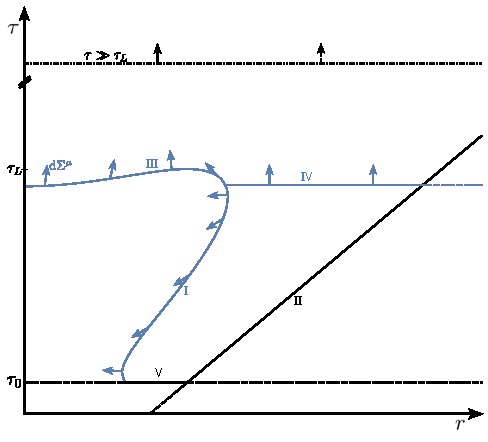
\includegraphics[width=0.4\linewidth]{images/FreezeOutSurface.pdf}
        \captionof{figure}{Freezeout surface in $\tau$-$r$-plane \cite{KirchnerEtAl_2023}.}
        \label{fig:FreezeOutSurface_rtau}
    \end{minipage}
}
The numerically determined shape of the freezeout surface is depicted in figure \ref{fig:FreezeOutSurface_rtau}. The intuitive picture of charges conserved under deformation of Cauchy surfaces is not enough to go from data on a hypersurface of constant lab time to the freezeout surface, since the latter undergoes a change from regions of timelike to spacelike normal vectors. Following the reasoning from \cite{KirchnerEtAl_2023}, we wish to apply Gauß law, taking care of the different signature compared to the usual version of Gauß law in Euclidean space. A calculation highlighting the difference between Euclidean and Minkowski signature is performed in Appendix \ref{sec:Apdx_GaußLawMinkowski}.

Assuming that the condensate has no contributions at large rapidities ${\eta\to\pm\infty}$, one can deform the hypersurface $\Sigma_t$ at large lab time ${t=\const}$ into a hypersurface of large Bjorken time $\Sigma_{\tau\gg\tau_L}$ at a $\tau$ much larger then the lifetime $\tau_L$ of the fireball, using Gauß law applied to the spacetime volume enclosed by these two Cauchy surfaces. There is no contribution from the $\tau$-axis, because the set of points where $r=0$ has vanishing 3-volume. Assuming further that the condensate contribution as a function in phase space $f_{\text{cond}}(x^\mu,\vec{p})$ vanishes on $\Sigma_{\rom{2}}$ and $\Sigma_{\rom{5}}$, i.e. is contained within the union of all light cones starting on the freezeout surface ${\Sigma_{\text{fo}}\equiv\Sigma_{\rom{1}}\cap\Sigma_{\rom{3}}}$, the contributions on $\Sigma_{\rom{4}}$ and $\Sigma_{\rom{1}}$ coincide. From intuition about the Euclidean version of Gauß law one would expect a change in sign, given the normal vectors on these surface oriented as in figure \ref{fig:FreezeOutSurface_rtau}. However, since $\Sigma_{\rom{1}}$ is a timelike hypersurface there is another sign-flip compared to the spacelike hypersurface $\Sigma_{\rom{4}}$.

To summarize, the hypersurface on which the inner products are computed can be changed according to
\begin{equation}
    (\phi_J,u_{\vec{p}}^{(*)})_{\Sigma_t}=(\phi_J,u_{\vec{p}}^{(*)})_{\Sigma_{\tau\gg\tau_L}}=(\phi_J,u_{\vec{p}}^{(*)})_{\Sigma_{\rom{3}}\cup\Sigma_{\rom{4}}}=(\phi_J,u_{\vec{p}}^{(*)})_{\Sigma_{\rom{3}}\cup\Sigma_{\rom{1}}}\equiv(\phi_J,u_{\vec{p}}^{(*)})_{\Sigma_{\text{fo}}}\,.
    \label{eq:InnerproductHypersurfaceDeformation}
\end{equation}

\section{Metric on the Freezeout Surface}
\label{sec:FOSurfaceMetric}

To evaluate the inner product \eqref{eq:InvariantInnterProduct} explicitly on the freezeout surface, we need to find the induced metric and surface element of the hypersurface as a submanifold of Minkowski space $\mathbb{R}^{(1,3)}$ using a standard procedure.

The freezeout hypersurface is parametrized as $\Sigma_{\text{fo}}=\{x^\mu\in\mathbb{R}^{(1,3)}\vert (\tau,r)=(\tau(\alpha),r(\alpha))\}$ with $\tau,r$ defined by the coordinate transformation \eqref{eq:BjorkenCoords_PositionSpace}. We will need the oriented surface normal $\dt\Sigma^\mu$ on this hypersurface. Recall the metric ${g_{\mu\nu}=\text{diag}(-1,1,\tau^2,r^2)}$ in Bjorken coordinates $(\tau,r,\eta,\varphi)$. Orthonormal tangent vectors on the freezeout hypersurface are ${(\hat\partial_\varphi)^\mu=(0,0,0,r^{-1})=r^{-1}(\partial_\varphi)^\mu}$, ${(\hat\partial_\eta)^\mu=(0,0,\tau^{-1},0)=\tau^{-1}(\partial_\eta)^\mu}$ and ${(\hat\partial_\alpha)^\mu=\sqrt{\vert r^{\prime 2}(\alpha)-\tau^{\prime 2}(\alpha)\vert}^{-1}(\tau^{\prime}(\alpha),r^{\prime}(\alpha),0,0)=D(\alpha)(\partial_\alpha)^\mu}$ with ${D(\alpha)=\sqrt{\vert r^{\prime 2}(\alpha)-\tau^{\prime 2}(\alpha)\vert}^{-1}}$. The projector on the hypersurface is
    \begin{multline}
        \gamma_{\mu\nu}=(\hat\partial_\varphi)_\mu(\hat\partial_\varphi)_\nu+(\hat\partial_\eta)_\mu(\hat\partial_\eta)_\nu+(\hat\partial_\alpha)_\mu(\hat\partial_\alpha)_\nu\\
        =\begin{pmatrix}
            D^2(\alpha)\tau^{\prime2}(\alpha)               & -D^2(\alpha)\tau^\prime(\alpha)r^\prime(\alpha) & 0      & 0   \\
            -D^2(\alpha)\tau^\prime(\alpha)r^\prime(\alpha) & D^2(\alpha)r^{\prime2}(\alpha)                  & 0      & 0   \\
            0                                               & 0                                               & \tau^2 & 0   \\
            0                                               & 0                                               & 0      & r^2
        \end{pmatrix}
    \end{multline}
The normal of the hypersurface, defined by its orthogonality to all tangent vectors, is ${n^\mu\equiv(\hat\partial_\alpha^\perp)^\mu=D(\alpha)(r^\prime(\alpha),\tau^\prime(\alpha),0,0)}$ and is timelike (spacelike) when ${r^\prime>\tau^\prime}$ (${r^\prime<\tau^\prime}$). Naturally ${\gamma_{\mu\nu}n^\nu=0}$. Using that
    \begin{equation}
        (\partial_\alpha)^\nu\gamma_{\mu\nu}(\partial_\alpha)^\mu=\begin{pmatrix}
            \tau^\prime \\r^\prime
        \end{pmatrix}^T\begin{pmatrix}
            -\tau^\prime \\
            r^\prime
        \end{pmatrix}=D^{-2}\,,
    \end{equation}
the induced hypersurface metric in coordinates ${x^i=(\alpha,\eta,\varphi)}$ reads
    \begin{equation}
        \gamma_{ij}=\text{diag}(D^{-2}(\alpha),\tau^2(\alpha),r^2(\alpha))
    \end{equation}
and the volume element is given by ${\dt\Sigma=\det(\gamma_{ij})\dt\alpha\dt\eta\dt\varphi=r(\alpha)\tau(\alpha) D^{-1}(\alpha)\dt\alpha\dt\eta\dt\varphi}$. The oriented surface element is 
\begin{equation}
        \dt\Sigma^\mu=n^\mu\dt\Sigma=r(\alpha)\tau(\alpha)(r^\prime(\alpha),\tau^\prime(\alpha),0,0)\dt\alpha\dt\eta\dt\varphi\,,
        \label{eq:FreezeoutSurface_SurfaceElementOriented}
\end{equation}
which is the main result from this section.

\section{Computing the Inner Product}

Coming back to the opening paragraph of this chapter, we now have all the building blocks to derive an explicit formula ready for numerical evaluation on the freezeout surface. The main equations to be linked together are now \eqref{eq:SpectraConversion}, \eqref{eq:NumberDensity}, \eqref{eq:SpectraFromSource} and \eqref{eq:SourceFieldRelation_InnerProduct} together with \eqref{eq:InnerproductHypersurfaceDeformation} and \eqref{eq:FreezeoutSurface_SurfaceElementOriented}.

The projection of the derivative onto the surface normal of $\Sigma_{\text{fo}}$  is (omitting the $\alpha$-dependence) 
\begin{equation}
    \dt\Sigma^\mu\partial_\mu=(r^\prime\partial_\tau+\tau^\prime\partial_r)\cdot r\tau\,\dt\alpha\dt\eta\dt\varphi\,.
\end{equation}
and there are a priori 3 integrals to be evaluated numerically. Making use of boost and rotational symmetry, one can perform the $\eta$- and $\varphi$-integration analytically. To do so, one can apply the following integrals related to Bessel functions: \url{https://dlmf.nist.gov/10.9}
\begin{subequations}
    % \begin{align}
    %     \int_0^{2\pi}\dt\varphi e^{\pm\imagu a\cos\varphi}&=\int_0^{2\pi}\big(\cos(a\cos\varphi)\pm\imagu\sin(a\cos\varphi)\big)=2\int_0^\pi\cos(a\cos\varphi)\\
    %     &=2\pi J_0(a)\\
    %     \int_{-\infty}^\infty\dt\eta e^{\pm\imagu a\cosh\eta}&=2\int_0^\infty\dt\eta\big(\cos(a\cosh\eta)\pm\imagu\sin(a\cosh\eta)\big)\\
    %     &=\pi\big(-Y_0(a)\pm\imagu J_0(a)\big)
    %     &=\pm\pi\imagu(J_0(a)\pm\imagu Y_0(a))=\begin{cases}
    %         +\pi\imagu H^{(1)}_0(a)&\text{for "+"}\\
    %         -\pi\imagu H^{(2)}_0(a)&\text{for "-"}
    %     \end{cases}
    % \end{align}
    \begin{equation}
        \int_0^{2\pi}\dt\varphi e^{\pm\imagu a\cos\varphi}=2\pi J_0(a)\,,\qquad
        \int_{-\infty}^\infty\dt\eta e^{\pm\imagu a\cosh\eta}=\pi\big(-Y_0(a)\pm\imagu J_0(a)\big)\,.
    \end{equation}
    Additionally to the integral representations, the following computation makes use of \url{https://dlmf.nist.gov/10.4}
    \begin{equation}
        J_{0}^\prime(x)=-J_1(x)\,,\qquad Y_0^\prime(x)=-Y_1(x)\,.
    \end{equation}
\end{subequations}
Straightforward substitution of the different formula into each other leads to the central result
\begin{multline}
    J(\pm p) =2\pi^2\int_0^\pi\dt\alpha\tau r\Bigg[(r^\prime\partial_\tau+\tau^\prime\partial_r)\phi(\tau,r)\Big[J_0(r p_T)\times\big(-Y_0(\tau\omega_T)\pm\imagu J_0(\tau\omega_T)\big)\Big]+\nonumber                                                                                             \\
                       + \phi(\tau,r)\Big[\tau^\prime\times p_T J_1(r p_T)\times\big(-Y_0(\tau\omega_T)\pm\imagu J_0(\tau\omega_T)\big)+\nonumber                                                                                                                                       \\
                       \qquad\phantom{+\phi(\tau,r)\Big[}+r^\prime\times J_0(r p_T)\times\omega_T\big(-Y_1(\tau\omega_T)\pm\imagu J_1(\tau\omega_T)\big)\Big]\Bigg]\,.
                       \label{eq:SpectrumFinalFormula}
\end{multline}
This can be evaluated numerically, once the shape of the freezeout surface is provided in the form of 2 functions $\tau(\alpha)$ and $r(\alpha)$, and the initial data ${\phi\vert_{\Sigma_{\text{fo}}}}$ and ${\dt\Sigma^\mu\partial_\mu\phi\vert_{\Sigma_{\text{fo}}}}$ is specified. The necessity of 2 scalar functions as initial data is consistent with the idea that a solution to the Klein-Gordon equation has 2 scalar function-valued degrees of freedom.

\begin{subequations}
    \begin{align}
        J(\pm p) & =-\int_{-\infty}^\infty\dt\eta\int_0^{2\pi}\dt\varphi\int_0^\pi\dt\alpha\tau r\Bigg[\phi(\tau,r)\big(r^\prime\overset{\leftrightarrow}{\partial_\tau}+\tau^\prime\overset{\leftrightarrow}{\partial_r}\big)e^{\pm\imagu(\tau \omega_T\cosh(\eta-\eta_p)-r p_T\cos(\varphi-\varphi_p))}\Bigg] \\
                           & =-\int_{-\infty}^\infty\dt\eta\int_0^{2\pi}\dt\varphi\int_0^\pi\dt\alpha\tau r\Bigg[\phi(\tau,r)\big(r^\prime\overset{\leftrightarrow}{\partial_\tau}+\tau^\prime\overset{\leftrightarrow}{\partial_r}\big)e^{\pm\imagu(\tau \omega_T\cosh\eta-r p_T\cos\varphi)}\Bigg]                      \\
                           & =-2\pi^2\int_0^\pi\dt\alpha\tau r\Bigg[\phi(\tau,r)(r^\prime\overset{\leftrightarrow}{\partial_\tau}+\tau^\prime\overset{\leftrightarrow}{\partial_r})\Big[J_0(r p_T)\times\big(-Y_0(\tau\omega_T)\pm\imagu J_0(\tau\omega_T)\big)\Big]\Bigg]                                                 \\
                           & =2\pi^2\int_0^\pi\dt\alpha\tau r\Bigg[(r^\prime\partial_\tau+\tau^\prime\partial_r)\phi(\tau,r)\Big[J_0(r p_T)\times\big(-Y_0(\tau\omega_T)\pm\imagu J_0(\tau\omega_T)\big)\Big]+\nonumber                                                                                             \\
                           & \phantom{=}\qquad + \phi(\tau,r)\Big[\tau^\prime\times p_T J_1(r p_T)\times\big(-Y_0(\tau\omega_T)\pm\imagu J_0(\tau\omega_T)\big)+\nonumber                                                                                                                                       \\
                           & \phantom{=}\qquad\phantom{+\phi(\tau,r)\Big[}+r^\prime\times J_0(r p_T)\times\omega_T\big(-Y_1(\tau\omega_T)\pm\imagu J_1(\tau\omega_T)\big)\Big]\Bigg]
    \end{align}
\end{subequations}

\begin{subequations}
    \begin{align}
        J(\overset{(-)}{+}p) & =-\int_{-\infty}^\infty\dt\eta\int_0^{2\pi}\dt\varphi\int_0^\pi\dt\alpha\tau r\Bigg[\phi(\tau,r)\big(r^\prime\overset{\leftrightarrow}{\partial_\tau}+\tau^\prime\overset{\leftrightarrow}{\partial_r}\big)e^{\overset{(-)}{+}\imagu(\tau \omega_T\cosh(\eta-\eta_p)-r p_T\cos(\varphi-\varphi_p))}\Bigg] \\
                           & =-\int_{-\infty}^\infty\dt\eta\int_0^{2\pi}\dt\varphi\int_0^\pi\dt\alpha\tau r\Bigg[\phi(\tau,r)\big(r^\prime\overset{\leftrightarrow}{\partial_\tau}+\tau^\prime\overset{\leftrightarrow}{\partial_r}\big)e^{\overset{(-)}{+}\imagu(\tau \omega_T\cosh\eta-r p_T\cos\varphi)}\Bigg]                      \\
                           & =\overset{(+)}{-}2\pi^2\imagu\int_0^\pi\dt\alpha\tau r\Bigg[\phi(\tau,r)(r^\prime\overset{\leftrightarrow}{\partial_\tau}+\tau^\prime\overset{\leftrightarrow}{\partial_r})\Big[J_0(r p_T)\times H_0^{\overset{(2)}{(1)}}(\tau\omega_T)\Big]\Bigg]                                                 \\
                           & =\overset{(-)}{+}2\pi^2\imagu\int_0^\pi\dt\alpha\tau r\Bigg[(r^\prime\partial_\tau+\tau^\prime\partial_r)\phi(\tau,r)\Big[J_0(r p_T)\times H_0^{\overset{(2)}{(1)}}(\tau\omega_T)\Big]+\nonumber                                                                                             \\
                           & \phantom{=}\qquad + \phi(\tau,r)\Big[\tau^\prime\times p_T J_1(r p_T)\times H_0^{\overset{(2)}{(1)}}(\tau\omega_T)+r^\prime\times J_0(r p_T)\times\omega_T H_1^{\overset{(2)}{(1)}}(\tau\omega_T)\Big]\Bigg]
    \end{align}
\end{subequations}



\section{Models for Initial Data}

The goal of this section is to find physically reasonable initial conditions for the condensate field distribution on the freezeout surface. Various approaches seem intuitive:
\begin{impt}[Possibilies to Fix Initial Data]{impt:InitialData}
\begin{enumerate}
    \item Prescribe fields and orhtogonal derivatives directly in the sense of an expansion on the freezeout surface (starting with constants, Gauß modes, etc.).
    \item Prescribe other physically accessible parameters like energy density $\epsilon$, pressure $p$ or fluid velocity $u^\mu$, and make contact with the fluid simulation.
    \item Prescribe fields as functions of $(\tau,r)$ during the fireball evolution, followed by restriction on $\Sigma_{\text{fo}}$.
\end{enumerate}
\end{impt}
Whereas the first approach imposes no constraints at all, some work must be put into the second approach. A key idea to assign physical quantitites of the QGP with the condensate field is by considering the conserved currents derived in section \ref{sec:ConservedCurrentsChirSym}. To be precise, we choose the (approximately) conserved vector and axial currents $J^\mu_{V,A}$ to be parallel to $u^\mu$, the only exceptional 4-vector in the fluid simulation. To simplify the ansatz further, we make the consistent assumption that not only the currents, but all gradients of the fields point in direction of $u^\mu$.

Making further contact with the fluid description of the QGP, we state here the Lagrangians and canonical energy-momentum tensors ${T^{\mu\nu}=2(\partial\mathscr{L}/\partial g_{\mu\nu})+g^{\mu\nu}\mathscr{L}}$ \cite{Weinberg_2008} for the real fields $\sigma$ and $\pi^0$, as well as the complex fields $\pi^\pm$. Using the expansion of the potential and Lagrangian density close to the vacuum, as performed in section \ref{sec:LinearSigmaModel}, they read
%%%% MORE DETAIL
%%%% MORE DETAIL
%%%% MORE DETAIL
\begin{subequations}
    \begin{align}
        % \mathscr{L}_\sigma&=-\frac{1}{2}(\partial_\mu\sigma)(\partial^\mu\sigma)-\frac{1}{2}m_\sigma^2\sigma^2\\
        T^{\mu\nu}_{\sigma}&=(\partial^\mu\sigma)(\partial^\nu\sigma)+g^{\mu\nu}\big(-\frac{1}{2}(\partial_\alpha\sigma)(\partial^\alpha\sigma)-\frac{1}{2}m_\pi^2(\pi^0)^2\big)\\
        % \mathscr{L}_{\pi^0}&=-\frac{1}{2}(\partial_\mu\pi^0)(\partial^\mu\pi^0)-\frac{1}{2}m_\pi^2(\pi^0)^2\\
        T^{\mu\nu}_{\pi^0}&=(\partial^\mu\pi^0)(\partial^\nu\pi^0)+g^{\mu\nu}\big(-\frac{1}{2}(\partial_\alpha\pi^0)(\partial^\alpha\pi^0)-\frac{1}{2}m_\pi^2(\pi^0)^2\big)\\
        % \mathscr{L}_{\pi^\pm}&=-(\partial_\mu\pi^+)(\overline{\partial_\mu\pi^+})-m_\pi^2\pi^+\overline{\pi^+}\\
        T^{\mu\nu}_{\pi^\pm}&=2(\partial^\mu\pi^+)(\overline{\partial^\nu\pi^+})+g^{\mu\nu}\big(-(\partial_\alpha\pi^+)(\overline{\partial^\alpha\pi^+})-m_\pi^2\pi^+\overline{\pi^+}\big)
    \end{align}
\end{subequations}
Following \cite{Weinberg_2008} the energy momentum tensor of a real scalar field $\varphi$ is
\begin{subequations}
    \begin{align}
        T_\varphi^{\mu\nu}&=-g^{\mu\nu}\big[\frac{1}{2}g^{\rho\sigma}(\partial_\rho\varphi)(\partial_\sigma\varphi)+V(\varphi)\big]+g^{\mu\rho}g^{\nu\sigma}(\partial_\rho\varphi)(\partial_\sigma\varphi)\\
        \epsilon&=-\frac{1}{2}g^{\rho\sigma}(\partial_\rho\varphi)(\partial_\sigma\varphi)+V(\varphi)\\
        p&=-\frac{1}{2}g^{\rho\sigma}(\partial_\rho\varphi)(\partial_\sigma\varphi)-V(\varphi)\\
        u^\mu&=-\big[-g^{\rho\sigma}(\partial_\rho\varphi)(\partial_\sigma\varphi)\big]^{-1/2}g^{\mu\nu}\partial_\nu\varphi
    \end{align}
\end{subequations}

\subsection{Real Fields}
\label{sec:FluidFromRealScalar}

Let $\varphi$ be a real scalar field, e.g. ${\varphi\in\{\sigma,\pi^0\}}$. The only availabe $4$-vector in the fluid theory is $u_\mu$. It is thus intuitive to try to identify the real-valued $4$vector ${\partial_\mu\varphi\sim u_\mu}$. Taking the normalization ${u_\mu u^\mu=-1}$ into account, one finds
\begin{equation}
    u_\mu=\frac{\partial_\mu\varphi}{\chi}\,,\qquad0<\chi^2\defeq-(\partial_\mu\varphi)(\partial^\mu\varphi)\,.
\end{equation}
This does not restrict the initial data enough to uniquely specify the resulting spectrum. We are left to prescribe two functions on the freezeout surface, namely $\varphi\vert_{\Sigma_{\text{fo}}}$ and $\chi\vert_{\Sigma_{\text{fo}}}$. This ansatz together with the result from \ref{sec:FOSurfaceMetric} yields for the normal projection of the field derivative
\begin{equation}
    \dt\Sigma^\mu\partial_\mu\varphi=\chi(r^\prime u_\tau+\tau^\prime u_r)\cdot r\tau\,\dt\alpha\dt\eta\dt\varphi\,.
\end{equation}

To restrict initial data further in a physically meaningful way, from the fluid theory we could try to match the energy density of the hypothetical superfluid
%%%% MORE DETAIL
%%%% MORE DETAIL
%%%% MORE DETAIL
% \begin{subequations}
%     \begin{align}
%         \epsilon_{s,\varphi}=u_\mu u_\nu T^{\mu\nu}_{\varphi}&=\frac{(\partial_\nu\varphi)(\partial_\mu\varphi)}{\chi^2}\Big((\partial^\mu\varphi)(\partial^\nu\varphi)+g^{\mu\nu}\big(-\frac{1}{2}(\partial_\alpha\varphi)(\partial^\alpha\varphi)-\frac{1}{2}m_\varphi^2(\varphi)^2\big)\Big)   \\
%         &=\chi^2-\big(\frac{1}{2}\chi^2-\frac{1}{2}m_\varphi^2\varphi^2\big)  \\
%         &=\frac{1}{2}\big(m_\varphi^2\varphi^2+\chi^2\big)
%     \end{align}
% \end{subequations}
\begin{equation}
    \epsilon_\varphi=\frac{1}{2}(m_\varphi^2\varphi^2+\chi^2)
\end{equation}
which changes along the freezeout surface as
    \begin{equation}
        \dt\epsilon=m_\varphi^2\varphi\dt\varphi+\chi\dt\chi=m_\varphi^2\varphi(\partial_\mu\varphi)\dt^\mu s+\chi\dt\chi=m_\varphi^2\varphi(\chi u_\mu)\dt^\mu s+\chi\dt\chi\,,
    \end{equation}
with ${\dt^\mu s=(\partial x^\mu)/(\partial\alpha)\dt\alpha\equiv(\tau^\prime,r^\prime)\dt\alpha}$ the displacement vector on the freezeout surface. For this prescription, the solution $\varphi$ on the freezout surface thus needs to fulfill the ODE
\begin{equation}
    \dt\varphi=\chi u_\mu\dt^\mu s\,,\quad
    \dt\chi=\frac{1}{\chi}\dt\epsilon-m_\varphi^2\varphi u_\mu\dt^\mu s
    \label{eq:InitialConditions_ODE}
\end{equation}
The solutions $(\varphi,\chi)$ of this ODE have 1 degree of freedom, e.g. the ratio of kinetic energy ${\epsilon_{\text{kin}}=(1/2)\chi^2}$ and ${\epsilon_{\text{pot}}=(1/2)m_\varphi^2\varphi^2}$ at $\alpha=0$. To be precise, choose ${r\in[0,1]}$ and set ${\epsilon_{\text{pot}}\big\vert_{\alpha=0}=r\epsilon}$ and ${\epsilon_{\text{kin}}\big\vert_{\alpha=0}=(1-r)\epsilon}$ to find initial values $\varphi\vert_{\alpha=0}$ and $\chi\vert_{\alpha=0}$.

\paragraph{The Sign of $u^\mu\partial_\mu\varphi$}

At freezeout it seems reasonable to expect a decreasing amplitude of the condensate density in direction of the fluid flow. In order to derive restrictions on the (functional) degrees of freedom from this observation, we make the following general statement:
\begin{impt}[Sign of Directional Derivative of $\varphi$]{impt:SignDVarphi}
    After a step of ${\dt\tau_E>0}$ in eigentime in direction of any 4-vector $v^\mu$ the change in amplitude is
    \begin{equation}
        \dt(\varphi^2)\sim\varphi\dt\varphi=\varphi(v^\mu\partial_\mu\varphi)\dt\tau_E.
    \end{equation}
    Thus, a decreasing (increasing) amplitude in direction $v^\mu$ corresponds to the choice ${\varphi(v^\mu\partial_\mu\varphi)\overset{(>)}{<}0}$.
\end{impt}

The 4-vector $u^\mu$ is timelike, ${u_\mu u^\mu=-1}$ and future oriented, $u^\tau>0$. Inserting the above ansatz ${\partial_\mu\varphi=\chi u_\mu}$ gives for the change in direction of the fluid velocity
\begin{equation}
    \dt\varphi=\chi u_\mu u^\mu\dt\tau_E=-\chi\dt\tau_E\,.
\end{equation}
In this case, ${\varphi\chi>0}$ is the appropiate choice for a decreasing density of the condensate in the locally comoving frame of the fluid. Note further that in the region on the freezeout surface where $r\approx 0$, the normal vector ${\dt\Sigma^\mu}$ is also timelike and future oriented and ${\dt\Sigma^\mu u_\mu<0}$. Therefore the projection ${\dt\Sigma^\mu\partial_\mu\varphi}$ has the opposite sign of $\chi$ in the corresponding range of $\alpha$.

\subsection{Complex Fields}

Complex fields have an additional real degree of freedom compared to real fields. Let $\phi$ be a complex field, e.g. $\phi\in\{\pi^+,\pi^-\}$, which can be conveniently represented by ${\phi=\sqrt{n}e^{\imagu\theta}}$, by 2 real parameters, a density $n$ and phase $\theta$. In the case of ${\phi=\pi^+}$, instead of the gradient ${\partial_\mu\phi}$, a real valued 4-vector to be identified with the 4-velocity is now the conserved current
%%%% MORE DETAIL
%%%% MORE DETAIL
%%%% MORE DETAIL
% \begin{align}
%     \epsilon^{a12}J_V^{a,\mu}&=(\partial_\mu\pi^1)\pi^2-(\partial_\mu\pi^2)\pi^1\\
%     &=\frac{\imagu}{2}\Big((\partial_\mu\pi^++\partial_\mu\pi^-)(\pi^+-\pi^-)-(\partial_\mu\pi^+-\partial_\mu\pi^-)(\pi^++\pi^-)\Big)\\
%     &=\imagu\Big(-(\partial_\mu\pi^+)\pi^-+(\partial_\mu\pi^-)\pi^+\Big)\\
%     &=\imagu\sqrt{n}\Big(-\big((\partial_\mu\sqrt{n})+\imagu\sqrt{n}(\partial_\mu\theta)\big)+\big((\partial_\mu\sqrt{n})-\imagu\sqrt{n}(\partial_\mu\theta)\big)\Big)\\
%     &=n(\partial_\mu\theta)
% \end{align}
\begin{equation}
    \epsilon^{a12}J_V^{a,\mu}=(\partial_\mu\pi^1)\pi^2-(\partial_\mu\pi^2)\pi^1=n(\partial_\mu\theta)
\end{equation}
This is precisely the conserved current derived from the $U(1)$ symmetry of phase rotations of $\pi^+$, or equivalently chiral vector rotations that interchange ${\pi^1\leftrightarrow\pi^2}$. The ansatz $J_V^{\mu,a}\sim u^\mu$ implies
\begin{equation}
    u_\mu=\frac{\partial_\mu\theta}{\chi_\theta}\,,\qquad 0<\chi_\theta^2\defeq-(\partial_\mu\theta)(\partial^\mu\theta)
\end{equation}
We already considered the more restrictive assumption $(\partial_\mu\pi^a)\sim u_\mu$, that leads to 
\begin{equation}
    u_\mu=\frac{\partial_\mu\sqrt{n}}{\chi_n}\,,\qquad 0<\chi_n^2\defeq-(\partial_\mu\sqrt{n})(\partial^\mu\sqrt{n})
\end{equation}
and a resulting energy density of
\begin{subequations}
    \begin{align}
        \epsilon_{s,\phi}=u_\mu u_\nu T^{\mu\nu}_{\phi}&=\frac{(\partial_\mu\theta)(\partial_\nu\theta)}{\chi_\theta^2}\Big(2(\partial^\mu\phi)(\partial^\nu\phi^*)+g^{\mu\nu}\big(-(\partial_\alpha\phi)(\partial^\alpha\phi^*)-m_\phi^2\phi\phi^*\big)\Big)\\
        &=n\chi_\theta^2+\chi^2_n+m_\phi^2n
    \end{align}
\end{subequations}
where the intermediate calculation
\begin{subequations}
    \begin{align}
        (\partial^\mu\phi)(\partial^\nu\phi^*)&=\big((\partial^\mu\sqrt{n})+\imagu\sqrt{n}(\partial^\mu\theta)\big)\big((\partial^\nu\sqrt{n})-\imagu\sqrt{n}(\partial^\nu\theta)\big)\\
        &=(\partial^\mu\sqrt{n})(\partial^\nu\sqrt{n})+n(\partial^\mu\theta)(\partial^\nu\theta)+\imagu\big(\sqrt{n}(\partial^\mu\theta)(\partial^\nu\sqrt{n})-\sqrt{n}(\partial^\nu\theta)(\partial^\mu\sqrt{n})\big)\\
        (\partial_\mu\phi)(\partial^\mu\phi^*)&=-\chi_n^2-n\chi_\theta^2
    \end{align}
\end{subequations}
is useful. Note how the imaginary part of this tensor is antisymmetric and thus does not contribute upon contraction with a symmetric tensor.

There is now an addition degree of freedom ($\chi_\theta$) compared to the real case. There is additional information given by the conserved vector current $J_v^{a,\mu}$. By means of the underlying assumption of parallelity of all gradients with the 4-velocity $u_\mu$, its conservation law reads
\begin{equation}
        0=\partial_\mu\big(n(\partial_\mu\theta)\big)=(\partial_\mu n)(\partial_\mu\theta)+n(\partial_\mu\partial^\mu\theta)=-\chi_\theta\chi_n+n\chi_\theta(\partial_\mu u^\mu)+nu^\mu(\partial_\mu\chi_\theta)
\end{equation}
Denote the 4-divergence of the 4-velocity by ${D=\partial_\mu u^\mu}$. Proceding as before, imposing ${\dt\epsilon_{s,\phi}=0}$ as well as the just derived identiy

Considering the fact that we have already proposed ways to initialize the real valued fields $\pi^1$, $\pi^2$, we could also simply construct $\pi^\pm=(1/\sqrt{2})(\pi^1\mp\imagu\pi^2)$ from these fields. Given $\partial_\mu\pi^{1,2}$, the density of the charged pion fields changes as
\begin{equation}
    \partial_\mu n=\partial_\mu(\pi^+\pi^-)=\frac{1}{2}\partial_\mu\big((\pi^1)^2+(\pi^2)^2\big)=(\partial_\mu\pi^1)\pi^1+(\partial_\mu\pi^2)\pi^2\,.
\end{equation}

\subsection{Condensate Evolution in the Fireball}

Let us investigate the possibility of an evolution process where the condensate density, i.e. the field amplitudes, rise during the fireball evolution with an easy-to-model ${(\tau,r)}$-dependence. A first guess might be a constant condensate amplitude as a function of the radial coordinate, which increases as a function of $\tau$. For real fields $\varphi$, we state
\begin{equation}
    \varphi(\tau,r)=(\tau-\tau_0)\overline{\varphi}
\end{equation}
with $\tau_0$ the parameter where the fluid description starts and $\overline{\varphi}$ a constant proportional to (the squareroot of) the energy density contained within the condensate field. This function is clearly only $\tau$-dependent and thus 
\begin{equation}
    \dt\Sigma^\mu\partial_\mu\varphi=\dt\Sigma^\tau\partial_\tau\varphi=r^\prime\overline{\varphi}\cdot r\tau\,\dt\alpha\dt\eta\dt\varphi
\end{equation}
\begin{equation}
    (r^\prime\partial_\tau+\tau^\prime\partial_r)\varphi(\tau,r)=r^\prime\overline{\varphi}
\end{equation}

\section{Examplary Spectra}
\label{sec:ExampleSpectra}

This section is aimed towards finding some intuition for the relation between particle mass, initial conditions and resulting spectra.

\subsection{Constant Initial Conditions}

First, investigate the spectrum of a real scalar field for constant values of the field an normal derivative. These have no clear physical motivation and we are only interested in the shape of the spectra, not their absolute values.\\
\debugbox{
    \begin{minipage}{\linewidth}
        \centering
        \debugbox{
            \begin{minipage}{0.4\linewidth}
                \centering
                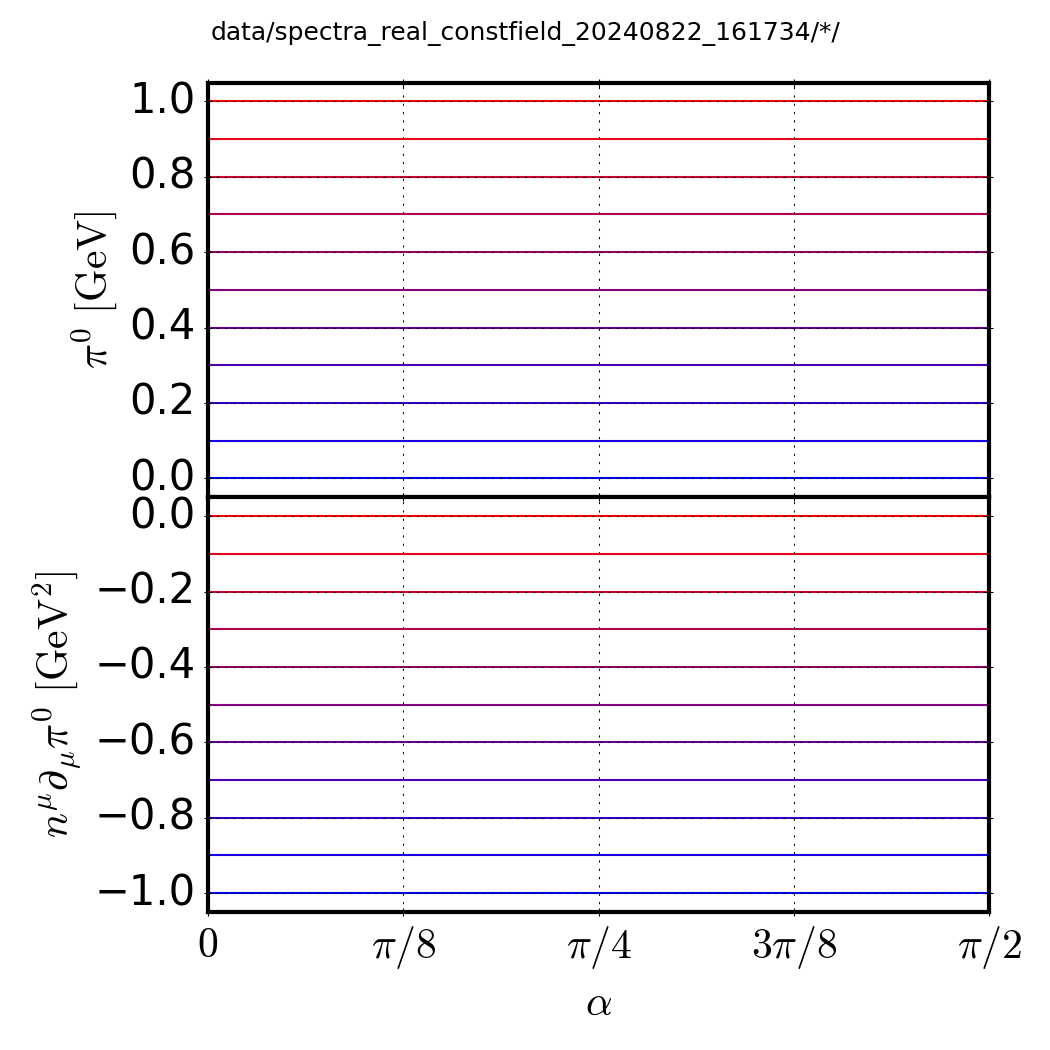
\includegraphics[width=\linewidth]{code/C++/DCCspec/data/images/spectra_real_constfield_20240822_161734_init.png}        
            \end{minipage}
        }
        \debugbox{
            \begin{minipage}{0.4\linewidth}
                \centering
                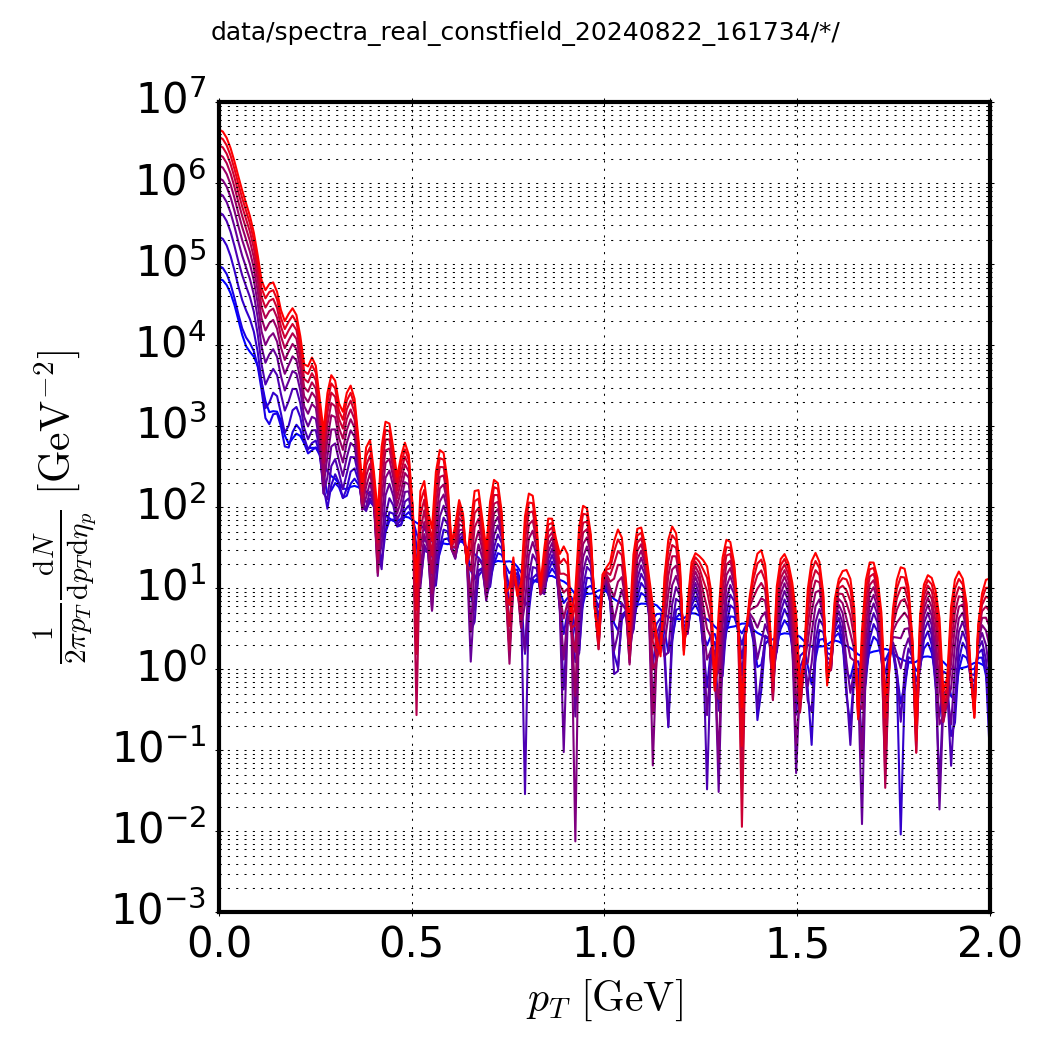
\includegraphics[width=\linewidth]{code/C++/DCCspec/data/images/spectra_real_constfield_20240822_161734_spec.png}        
            \end{minipage}
        }
    \end{minipage}
}
Spectra from field configurations of high ratio ${\Big\vert\frac{\text{amplitude}}{\text{derivative}}\Big\vert}$ tend to be more "bumpy"/oscillate quicker in momentum space. Investigating formula \eqref{eq:SpectrumFinalFormula} this is probably due to the fact that $\phi$ and $\partial\phi$ are multiplied with Bessel functions of different order, that exhibit different limiting behaviour at relevant points in the integral, namely at ${\tau(\alpha)\to0}$ or ${r(\alpha)\to0}$. These configurations are also well suited to test separately the impact of the mass parameter in the spectrum computation, keeping the initial conditions fixed.\\
\debugbox{
    \begin{minipage}{\linewidth}
        \centering
        \debugbox{
            \begin{minipage}{0.4\linewidth}
                \centering
                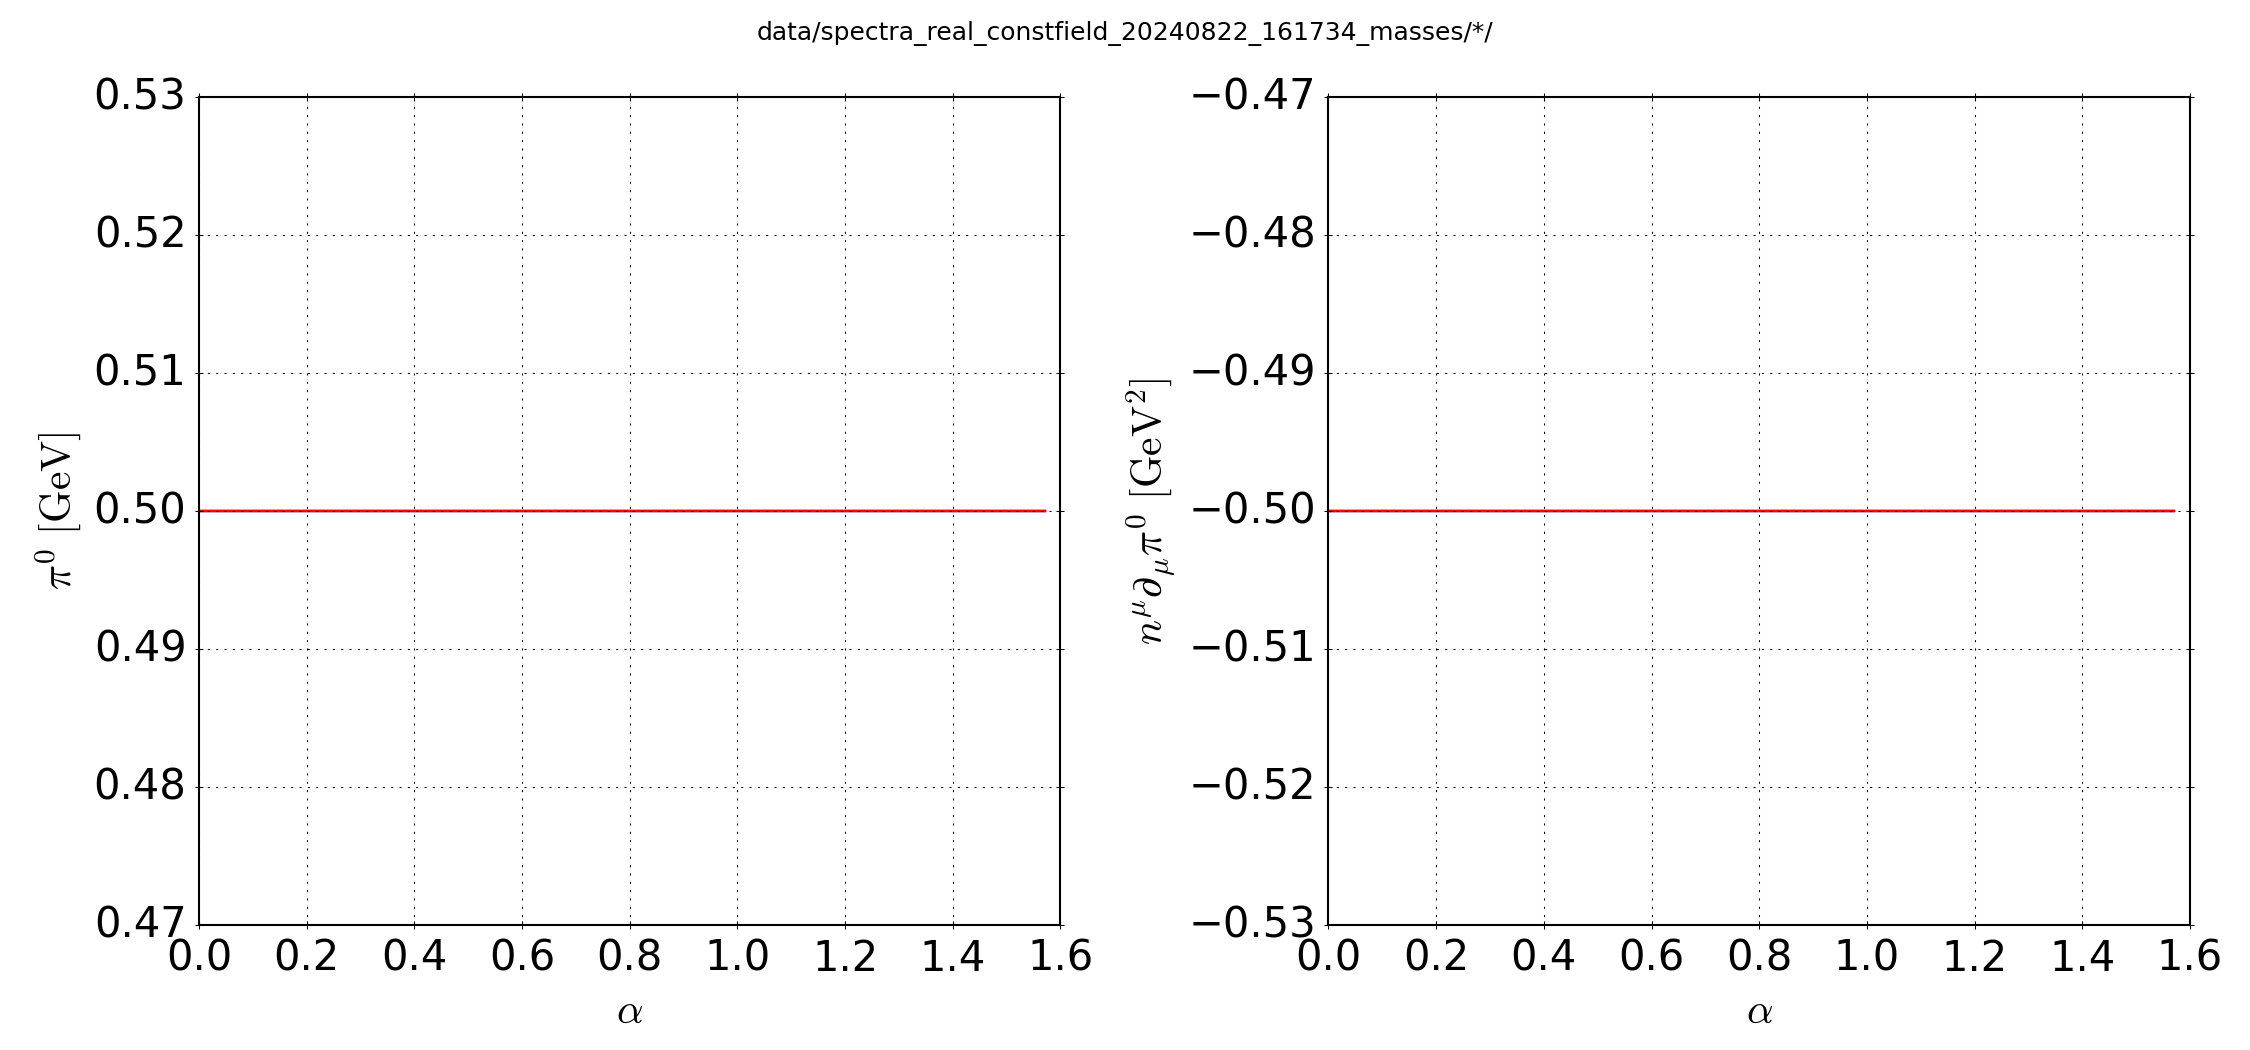
\includegraphics[width=\linewidth]{code/C++/DCCspec/data/images/spectra_real_constfield_20240822_161734_masses_init.png}        
            \end{minipage}
        }
        \debugbox{
            \begin{minipage}{0.4\linewidth}
                \centering
                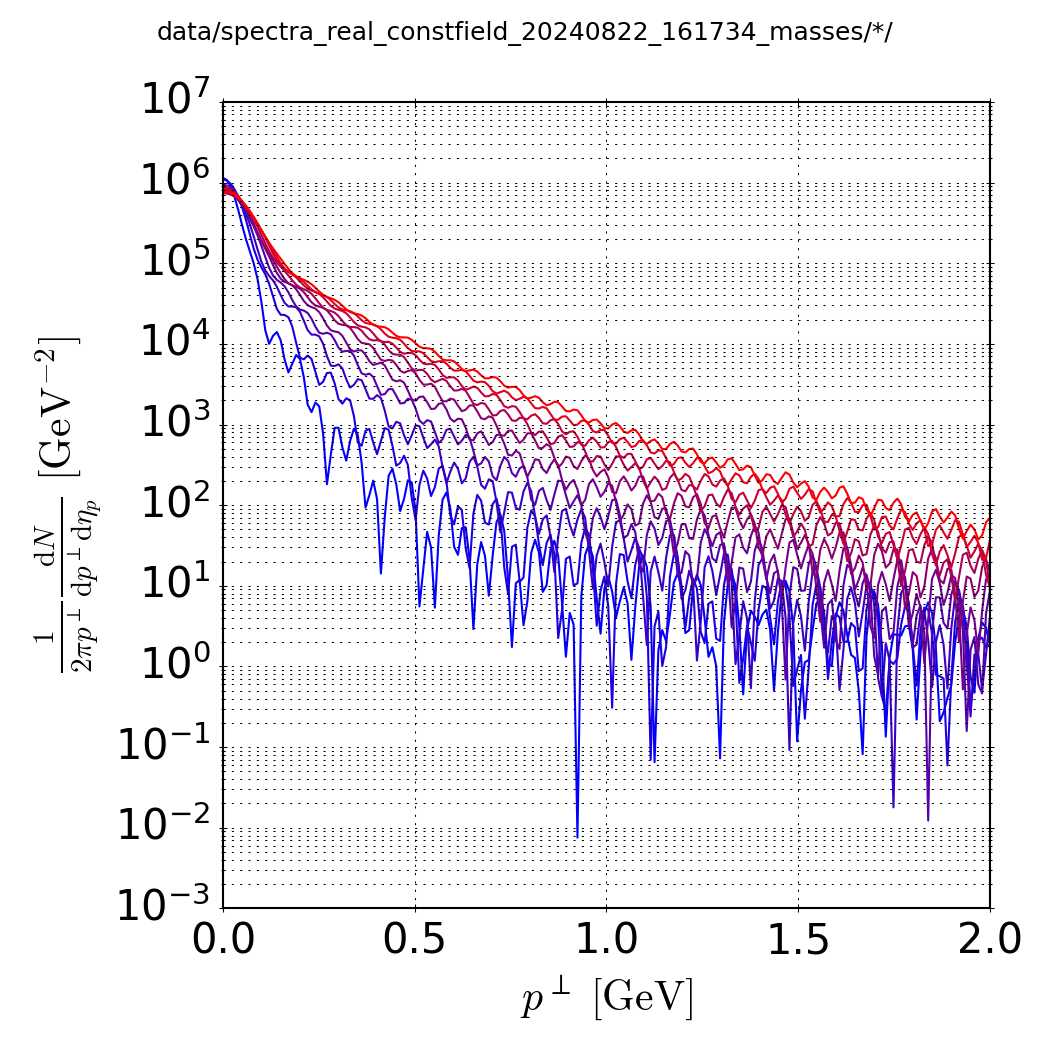
\includegraphics[width=\linewidth]{code/C++/DCCspec/data/images/spectra_real_constfield_20240822_161734_masses_spec.png}        
            \end{minipage}
        }
    \end{minipage}
}
The displayed graphs correspond to particle masses from 0.14 GeV (blue) to 0.8 GeV (red). Together with the scale on which the freezeout surface varies, the particle mass sets the main scale/width of the spectrum, as is evident from the combinations ${rp_T}$ and ${\tau\omega_T}$ appearing in formula \eqref{eq:SpectrumFinalFormula}. An increasing particle mass leads to a wider spectrum and has a similar effect as artificially decreasing the length scale of the freezeout surface.

\subsection{Constant Energy Density}

Next, test the aforementioned $\epsilon=\const$ prescription of defining initial data, which yields a 1-parameter family of initial field configurations. As previously described, the free parameter chosen here is the ratio ${r=\epsilon_{\text{pot}}/\epsilon}$ of potential to full energy density at ${\alpha=0}$. The energy density of the condensate is estimated by an arbitrary amount of $0.1\%$ of the energy density ${\epsilon_{\text{hydro}}\approx 0.16\,\mathrm{GeV}/(\mathrm{fm}^3)}$ of the hydro simulation.\\
\debugbox{
    \begin{minipage}{\linewidth}
        \centering
        \debugbox{
            \begin{minipage}{0.4\linewidth}
                \centering
                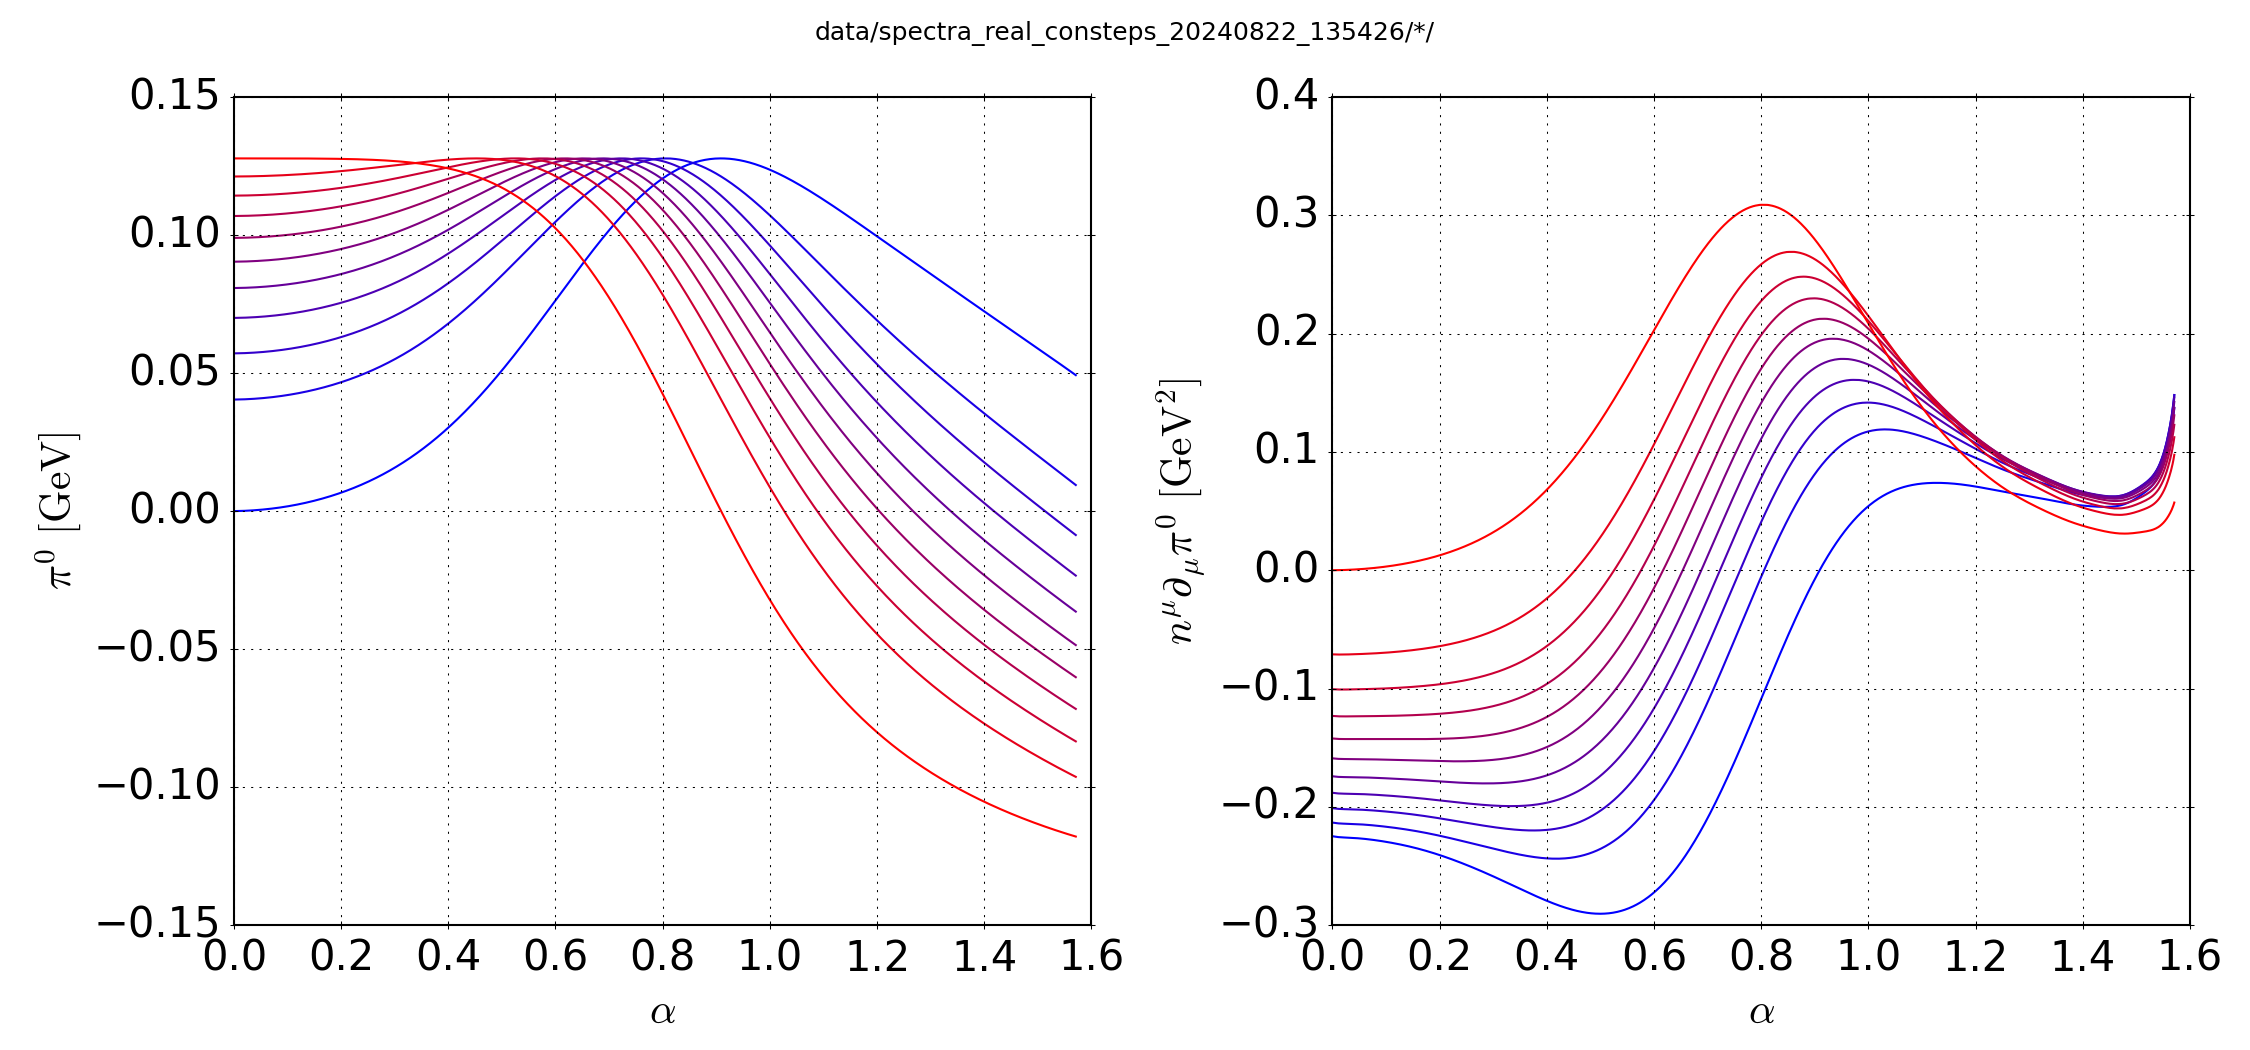
\includegraphics[width=\linewidth]{code/C++/DCCspec/data/images/spectra_real_consteps_20240822_135426_init.png}        
            \end{minipage}
        }
        \debugbox{
            \begin{minipage}{0.4\linewidth}
                \centering
                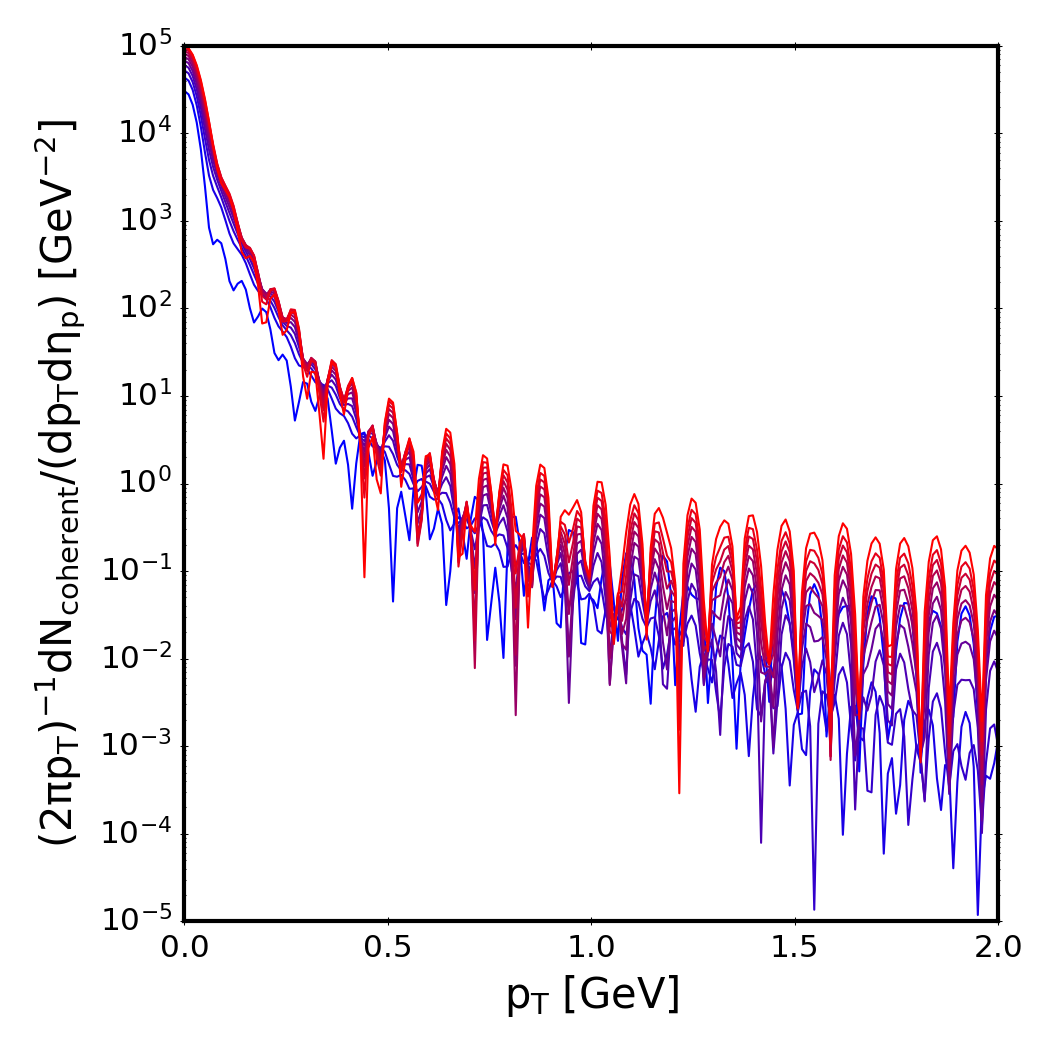
\includegraphics[width=\linewidth]{code/C++/DCCspec/data/images/spectra_real_consteps_20240822_135426_spec.png}        
            \end{minipage}
        }
        \captionof{figure}{Initial conditions (left) and resulting spectra (right) for constant energy density on the freezeout, using $m_\pi=0.140\,\text{GeV}$.}
        \label{fig:SpecRealConstEps_m140}
    \end{minipage}
}
The red graphs represent field configurations that are approximately constant on the ${\tau\approx\const}$ section of the freezeout surface. They seem to generate a distinct "break" in the spectrum, where the average slope (in the log scale) changes abruptly.

As before, let us also change the mass in this scenario. Now, the mass further influences the initial conditions and lead to more oscillations along the freezeout surface. The following graphs range from 0.14 GeV to 1 GeV particle mass.

\debugbox{
    \begin{minipage}{\linewidth}
        \centering
        \debugbox{
            \begin{minipage}{0.4\linewidth}
                \centering
                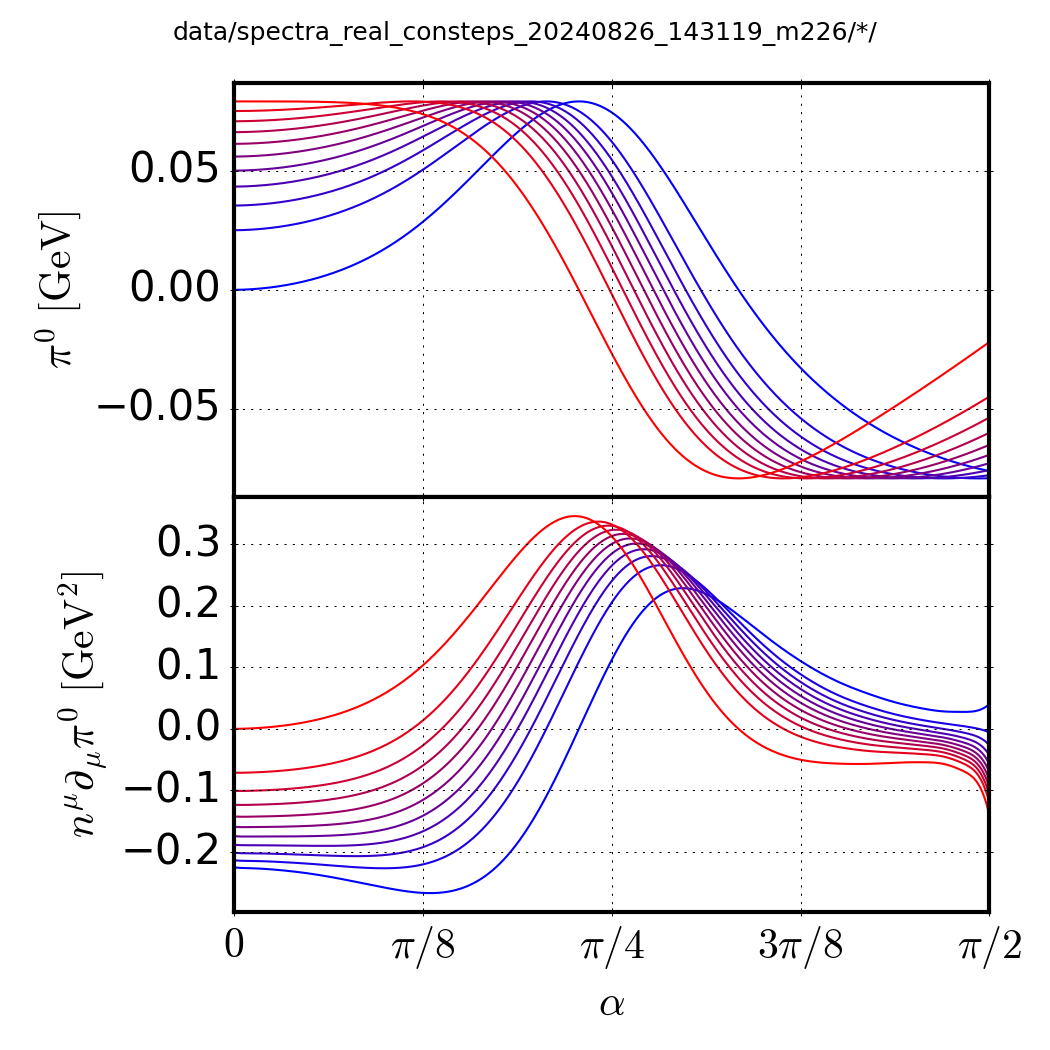
\includegraphics[width=\linewidth]{code/C++/DCCspec/data/images/spectra_real_consteps_20240826_143119_m226_init.png}        
            \end{minipage}
        }
        \debugbox{
            \begin{minipage}{0.4\linewidth}
                \centering
                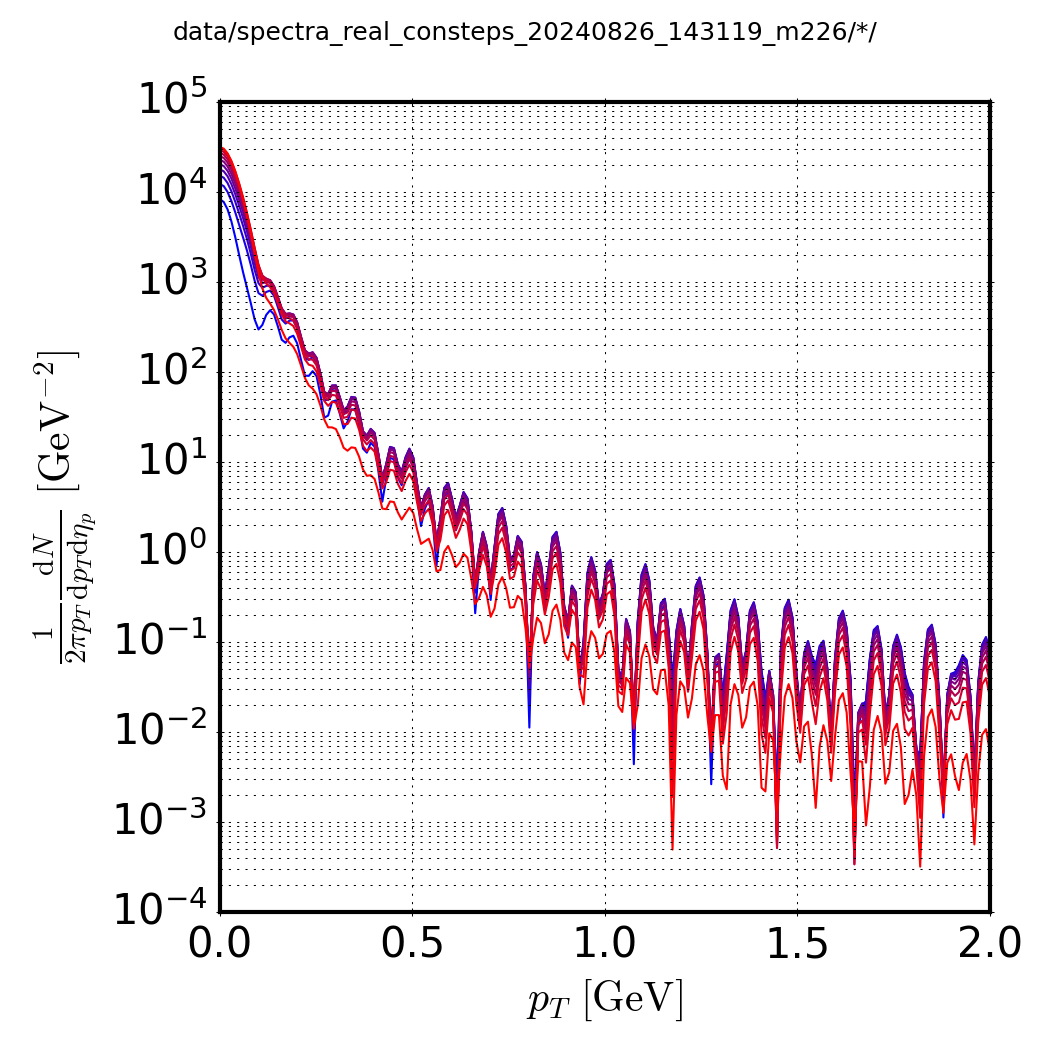
\includegraphics[width=\linewidth]{code/C++/DCCspec/data/images/spectra_real_consteps_20240826_143119_m226_spec.png}        
            \end{minipage}
        }
        \captionof{figure}{Initial conditions (left) and resulting spectra (right) for constant energy density on the freezeout, using $m_\pi=0.226\,\text{GeV}$.}
        \label{fig:SpecRealConstEps_m226}
    \end{minipage}
}

\debugbox{
    \begin{minipage}{\linewidth}
        \centering
        \debugbox{
            \begin{minipage}{0.4\linewidth}
                \centering
                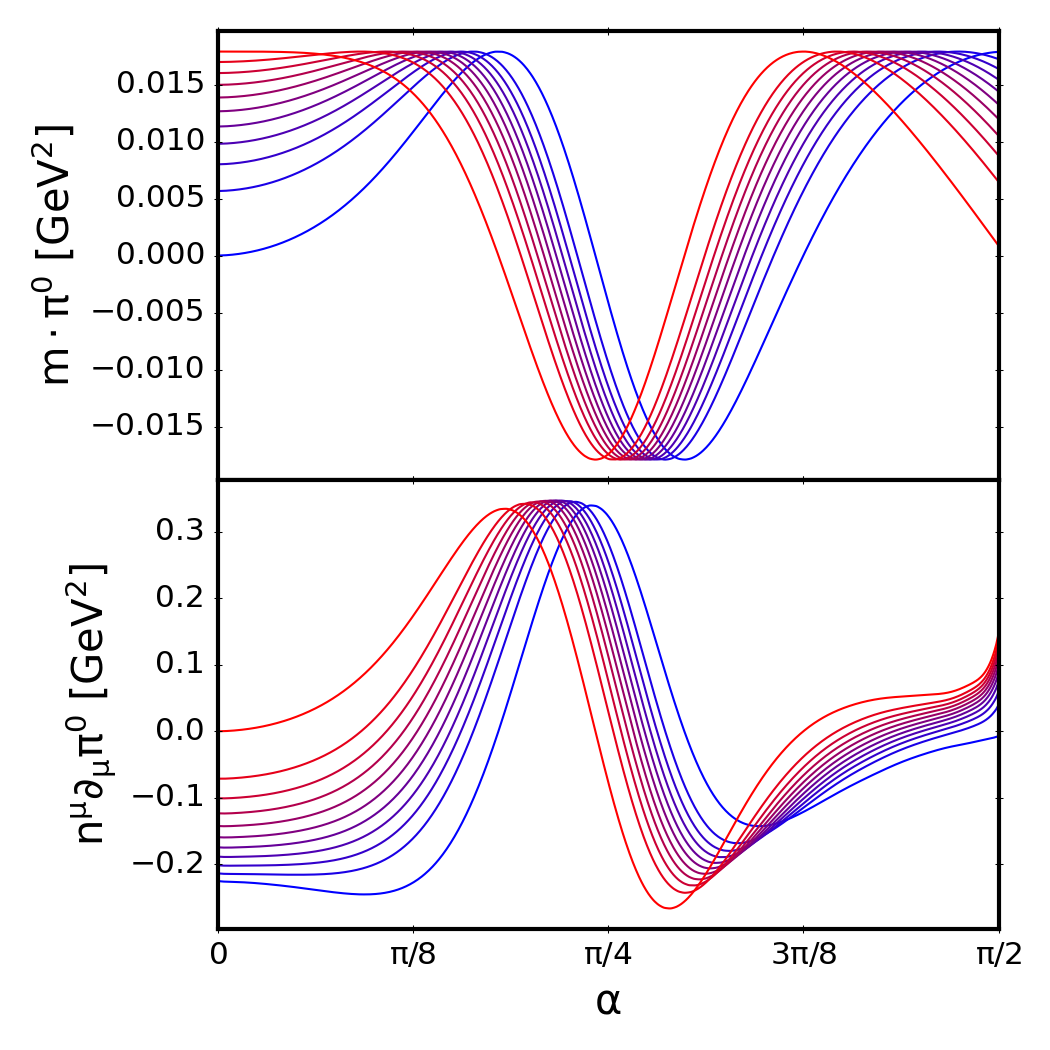
\includegraphics[width=\linewidth]{code/C++/DCCspec/data/images/spectra_real_consteps_20240826_143151_m398_init.png}        
            \end{minipage}
        }
        \debugbox{
            \begin{minipage}{0.4\linewidth}
                \centering
                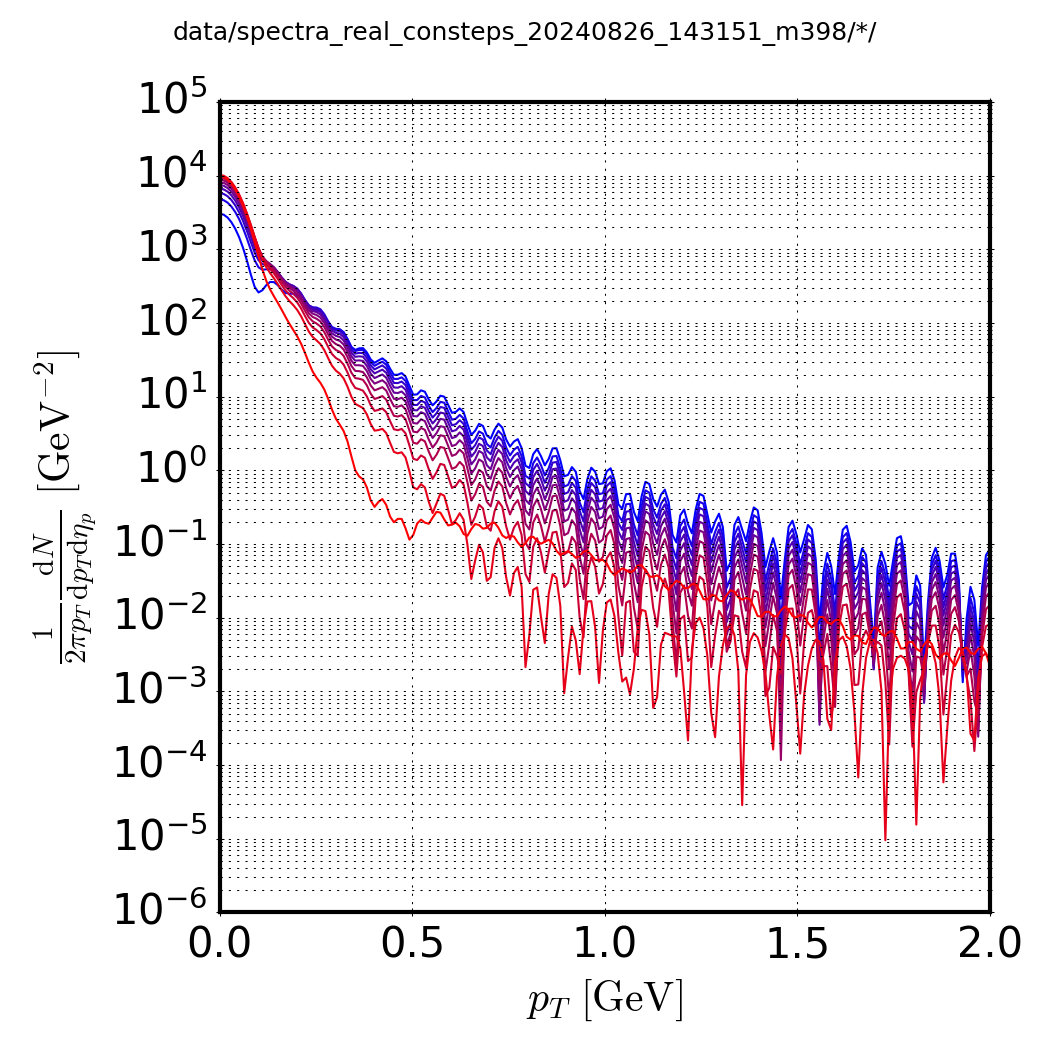
\includegraphics[width=\linewidth]{code/C++/DCCspec/data/images/spectra_real_consteps_20240826_143151_m398_spec.png}        
            \end{minipage}
        }
        \captionof{figure}{Initial conditions (left) and resulting spectra (right) for constant energy density on the freezeout, using $m_\pi=0.398\,\text{GeV}$.}
        \label{fig:SpecRealConstEps_m398}
    \end{minipage}
}

\debugbox{
    \begin{minipage}{\linewidth}
        \centering
        \debugbox{
            \begin{minipage}{0.4\linewidth}
                \centering
                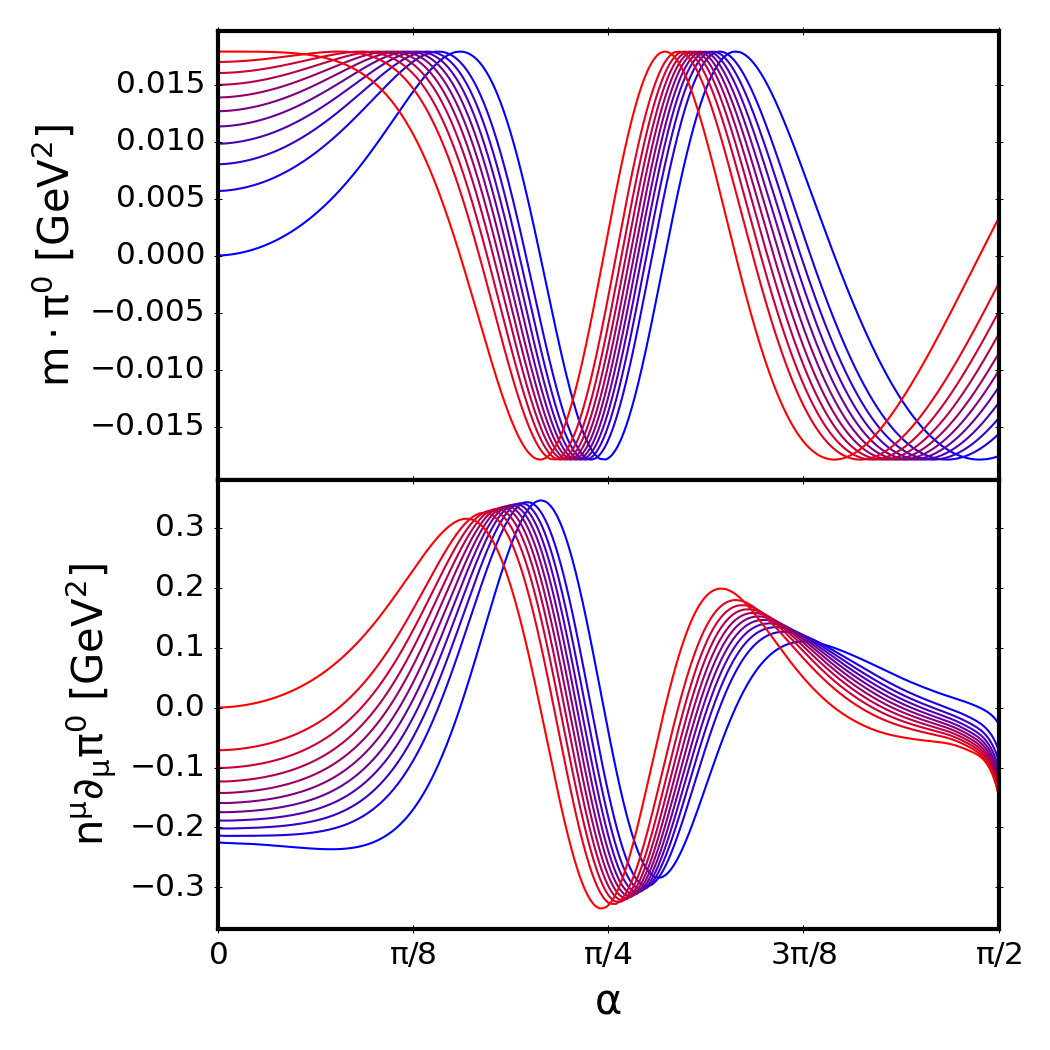
\includegraphics[width=\linewidth]{code/C++/DCCspec/data/images/spectra_real_consteps_20240826_143224_m570_init.png}        
            \end{minipage}
        }
        \debugbox{
            \begin{minipage}{0.4\linewidth}
                \centering
                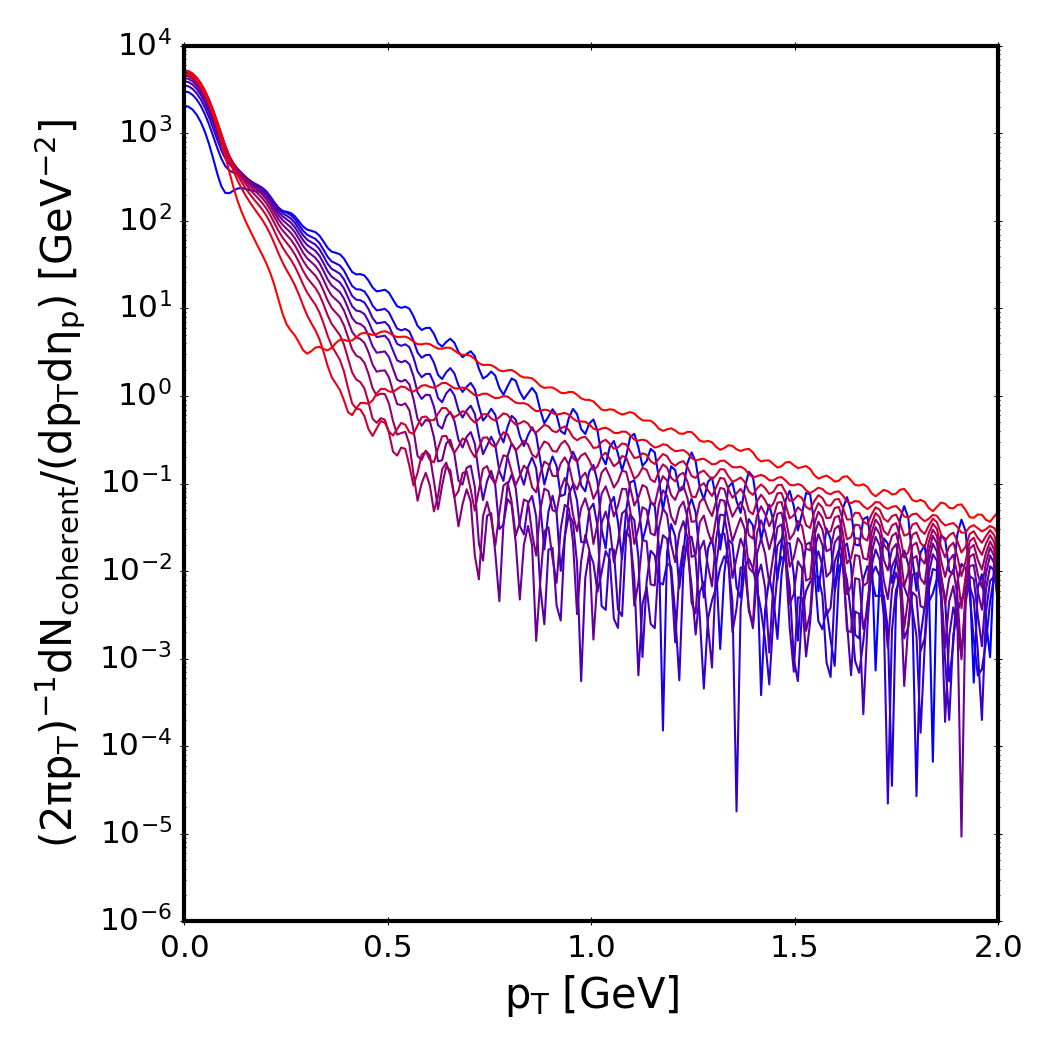
\includegraphics[width=\linewidth]{code/C++/DCCspec/data/images/spectra_real_consteps_20240826_143224_m570_spec.png}        
            \end{minipage}
        }
        \captionof{figure}{Initial conditions (left) and resulting spectra (right) for constant energy density on the freezeout, using $m_\pi=0.570\,\text{GeV}$.}
        \label{fig:SpecRealConstEps_m570}
    \end{minipage}
}

\debugbox{
    \begin{minipage}{\linewidth}
        \centering
        \debugbox{
            \begin{minipage}{0.4\linewidth}
                \centering
                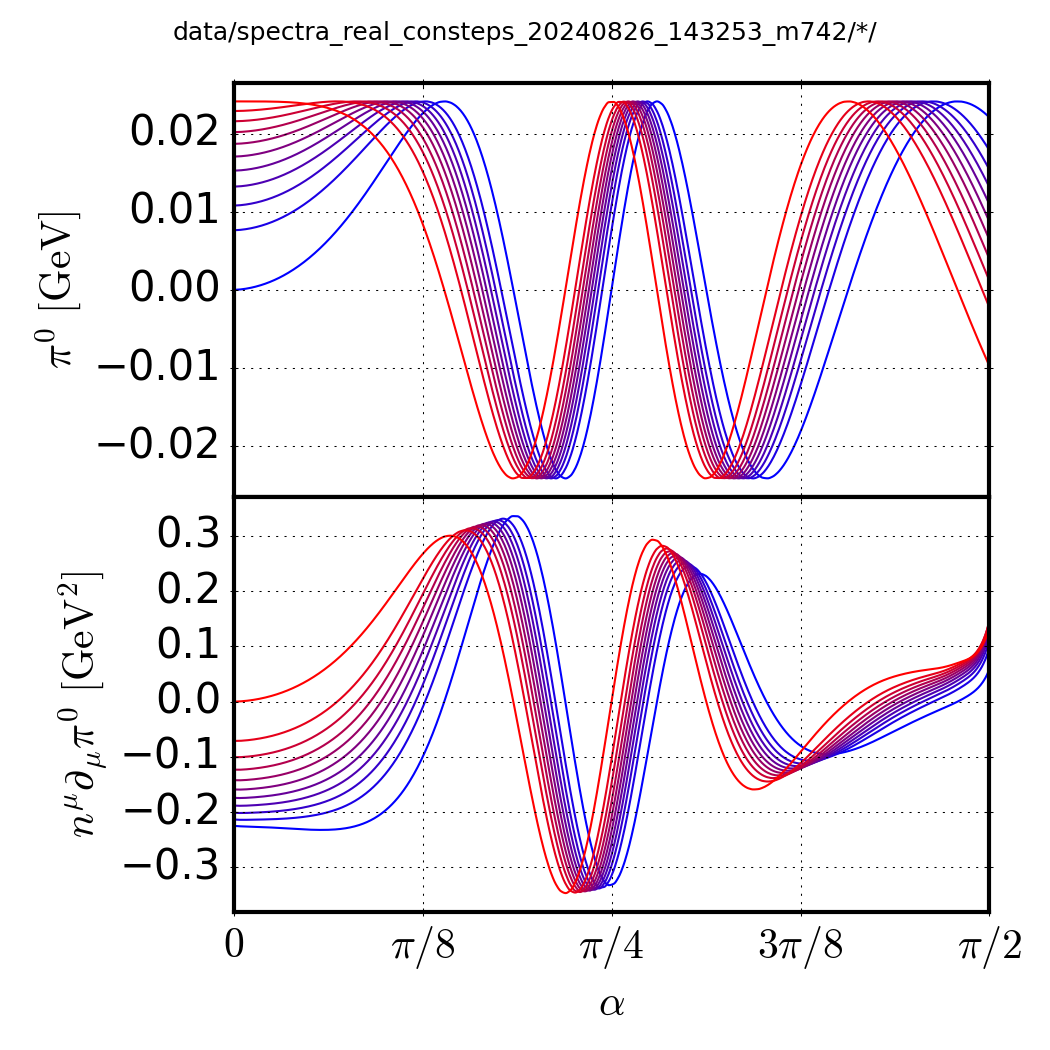
\includegraphics[width=\linewidth]{code/C++/DCCspec/data/images/spectra_real_consteps_20240826_143253_m742_init.png}        
            \end{minipage}
        }
        \debugbox{
            \begin{minipage}{0.4\linewidth}
                \centering
                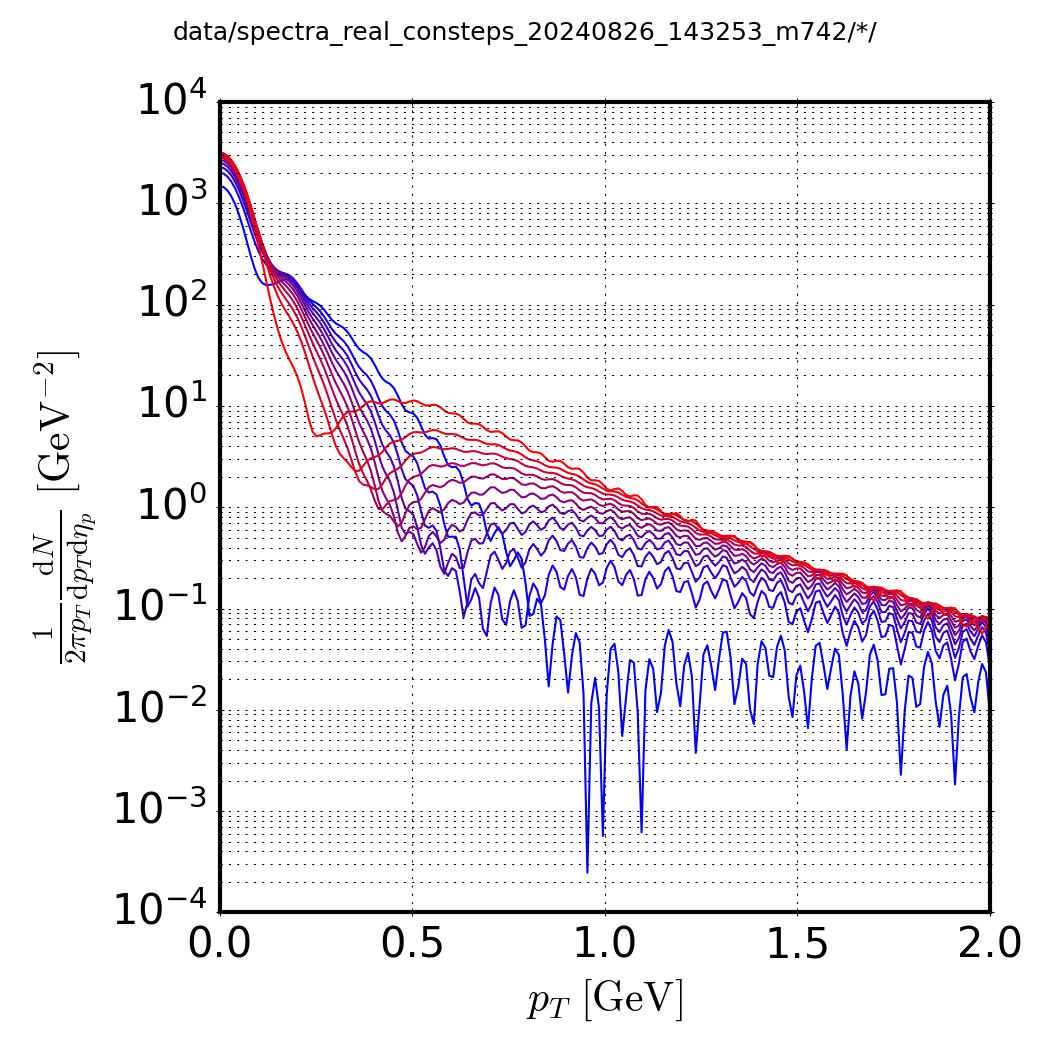
\includegraphics[width=\linewidth]{code/C++/DCCspec/data/images/spectra_real_consteps_20240826_143253_m742_spec.png}        
            \end{minipage}
        }
        \captionof{figure}{Initial conditions (left) and resulting spectra (right) for constant energy density on the freezeout, using $m_\pi=0.742\,\text{GeV}$.}
        \label{fig:SpecRealConstEps_m742}
    \end{minipage}
}

\debugbox{
    \begin{minipage}{\linewidth}
        \centering
        \debugbox{
            \begin{minipage}{0.4\linewidth}
                \centering
                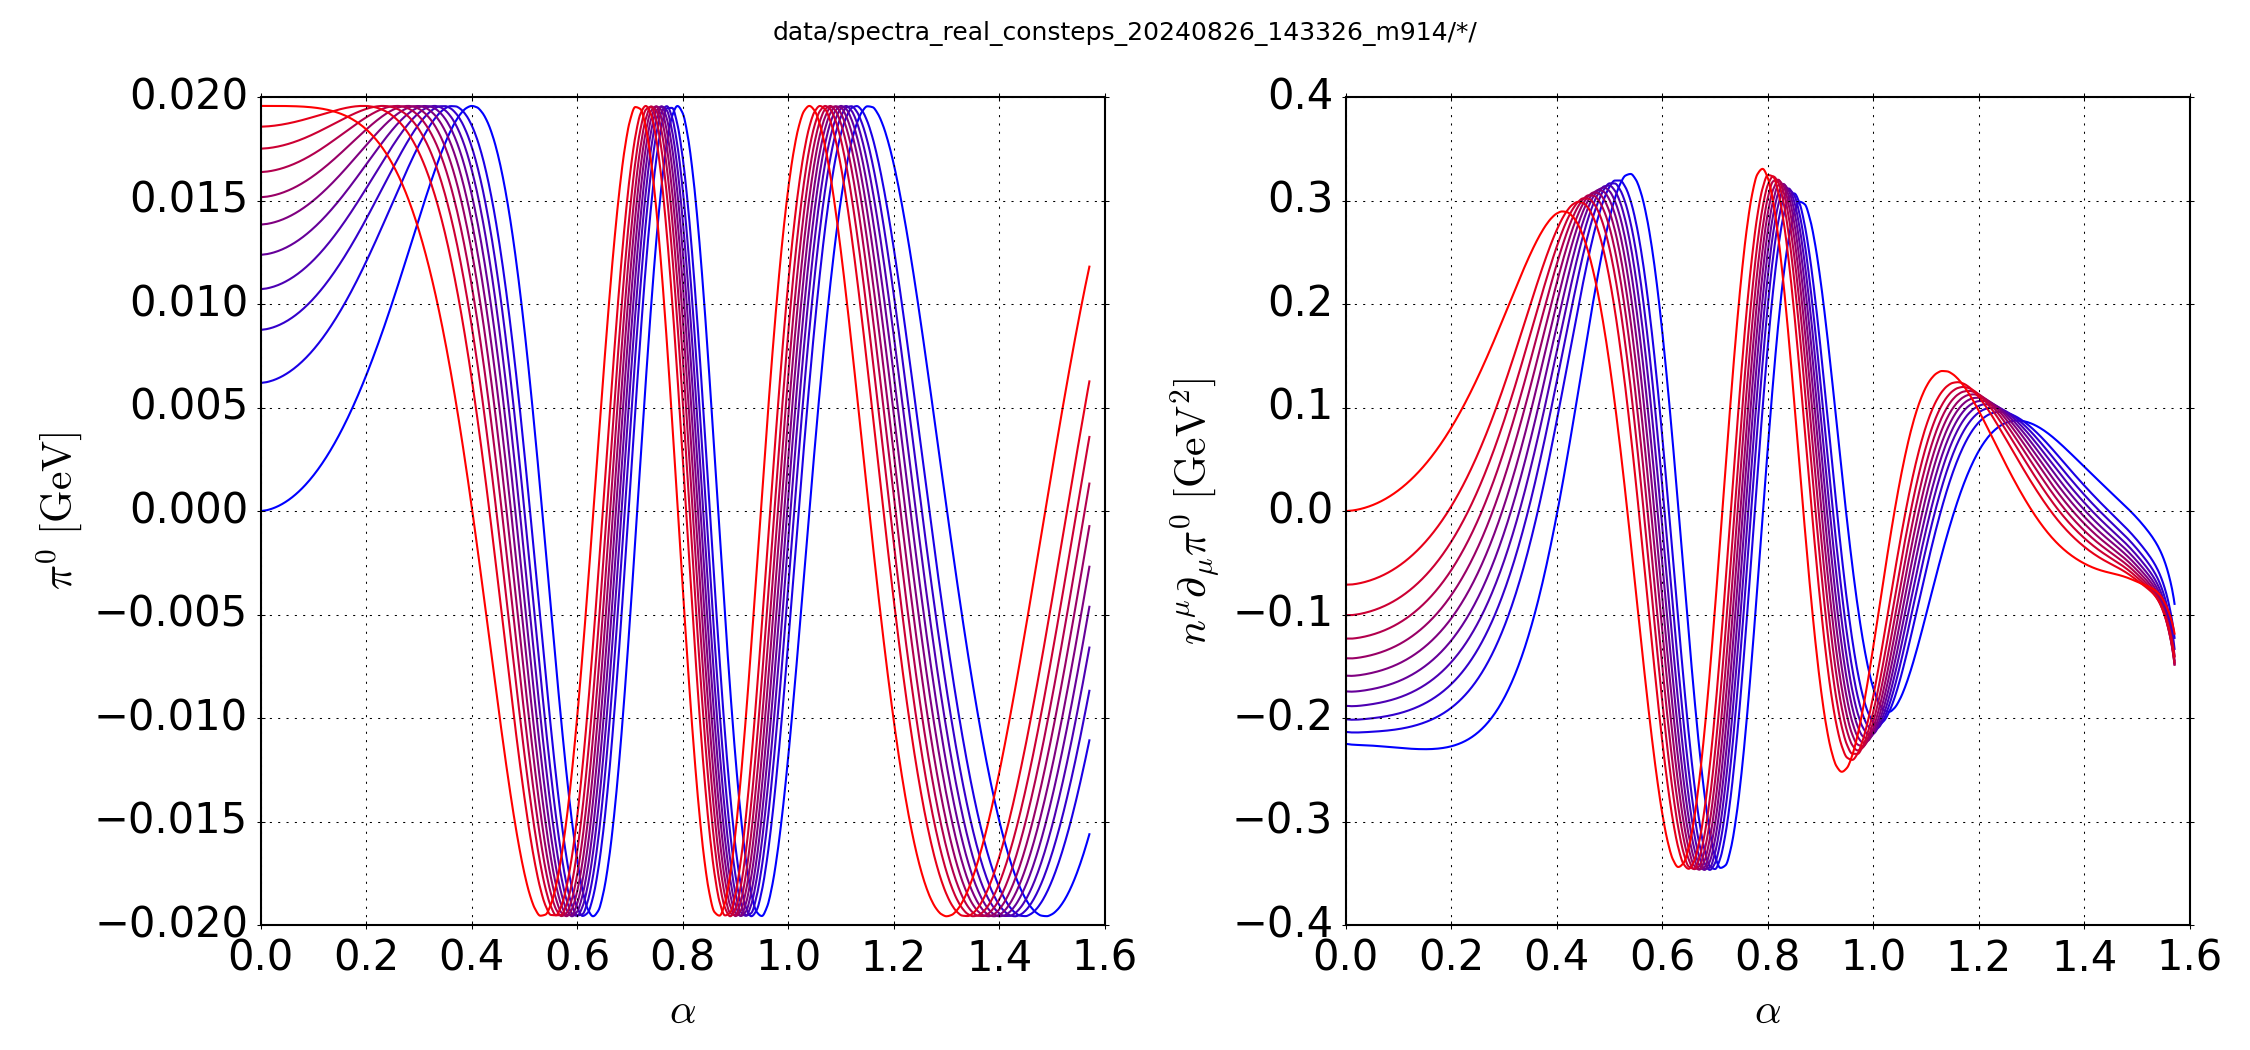
\includegraphics[width=\linewidth]{code/C++/DCCspec/data/images/spectra_real_consteps_20240826_143326_m914_init.png}        
            \end{minipage}
        }
        \debugbox{
            \begin{minipage}{0.4\linewidth}
                \centering
                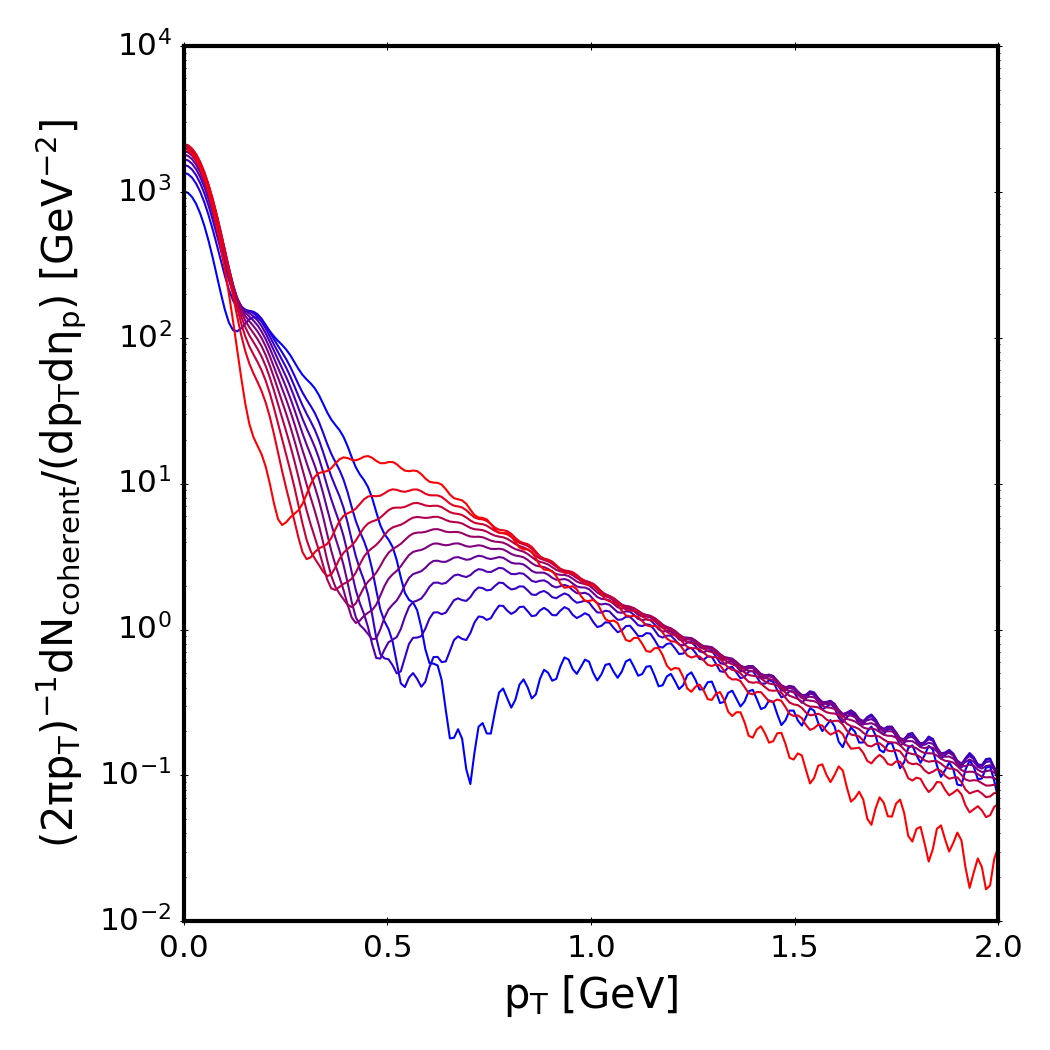
\includegraphics[width=\linewidth]{code/C++/DCCspec/data/images/spectra_real_consteps_20240826_143326_m914_spec.png}        
            \end{minipage}
        }
        \captionof{figure}{Initial conditions (left) and resulting spectra (right) for constant energy density on the freezeout, using $m_\pi=0.914\,\text{GeV}$.}
        \label{fig:SpecRealConstEps_m914}
    \end{minipage}
}

\debugbox{
    \begin{minipage}{\linewidth}
        \centering
        \debugbox{
            \begin{minipage}{0.4\linewidth}
                \centering
                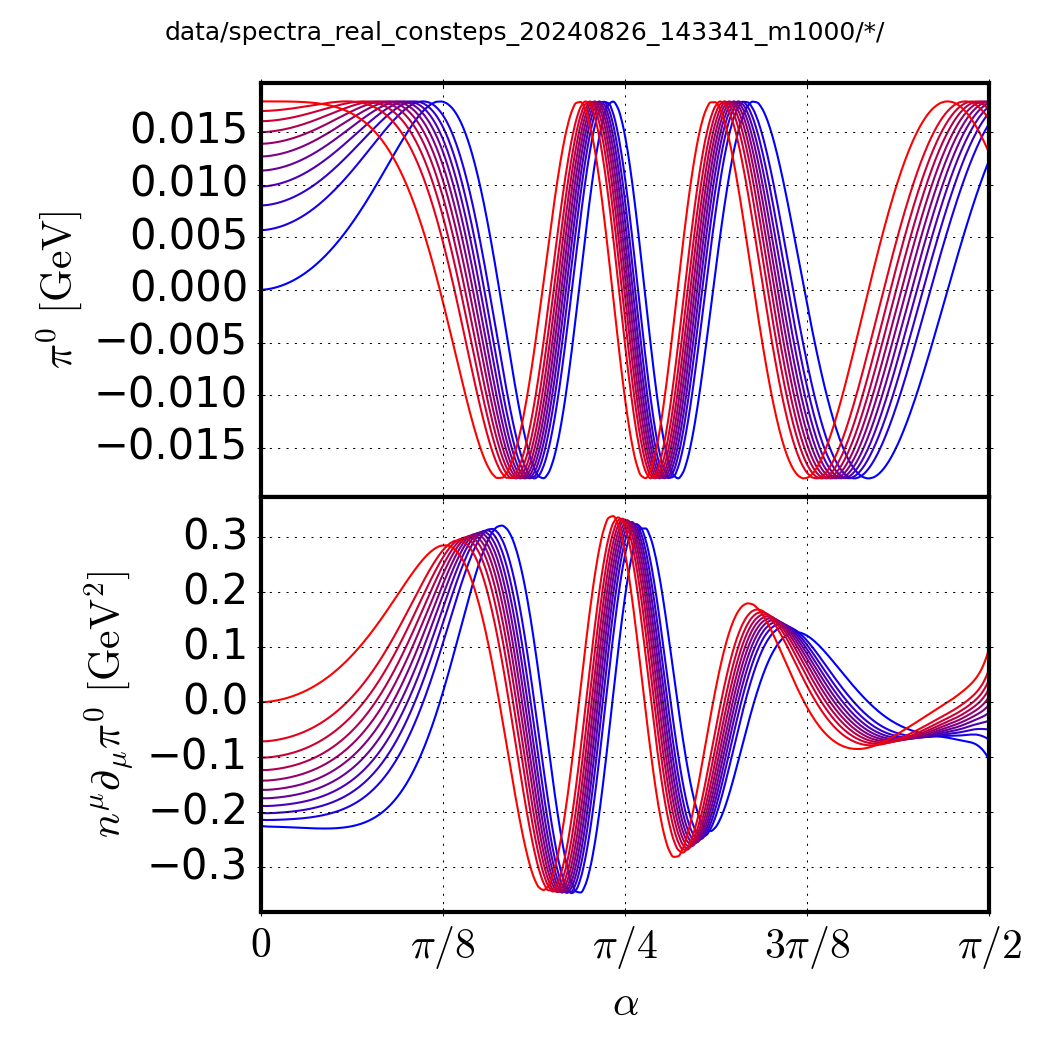
\includegraphics[width=\linewidth]{code/C++/DCCspec/data/images/spectra_real_consteps_20240826_143341_m1000_init.png}        
            \end{minipage}
        }
        \debugbox{
            \begin{minipage}{0.4\linewidth}
                \centering
                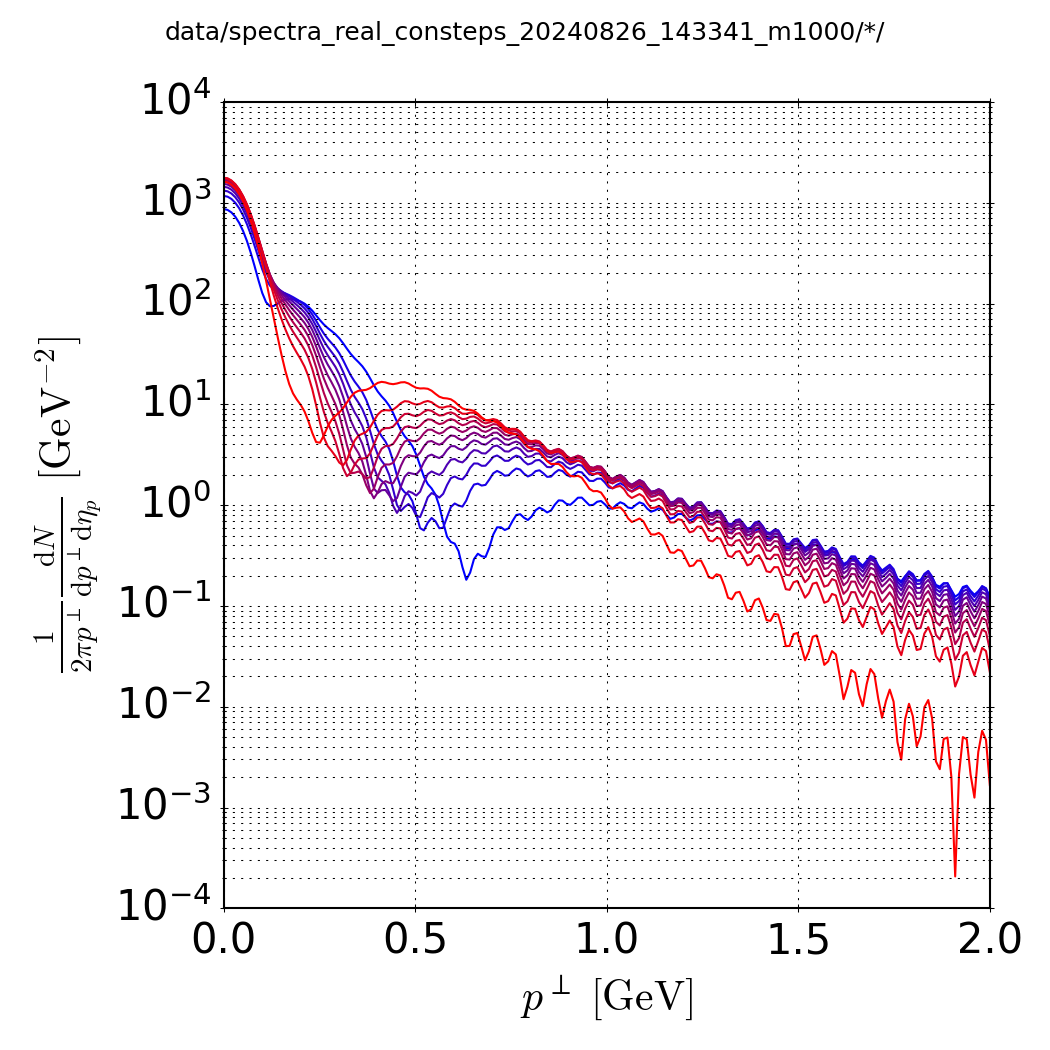
\includegraphics[width=\linewidth]{code/C++/DCCspec/data/images/spectra_real_consteps_20240826_143341_m1000_spec.png}        
            \end{minipage}
        }
        \captionof{figure}{Initial conditions (left) and resulting spectra (right) for constant energy density on the freezeout, using $m_\pi=1\,\text{GeV}$.}
        \label{fig:SpecRealConstEps_m1000}
    \end{minipage}
}
With increasing mass, one observers increasing width of the spectrum - as it was already observed and discussed in the last paragraph - as well as a second dominant bump away from $p_T=0\,\text{GeV}$, namely roughly at the particle mass. This fits the expectation of a general Fourier transformation picking up the dominant frequencies present in a field configuration. Requesting ${\epsilon=\const}$ and a hypothetically fixed value of the projection ${u_\mu\dt^\mu s}$, equation \eqref{eq:InitialConditions_ODE} becomes simply a coupled ODE describing harmonic oscillation with frequency $m_\varphi$. Therefore, the Fourier transform has a peak at that frequency, modulated with the effects of the non-trivial hypersurface geometry. The precise way in which the geometry affects this behaviour of the Fourier transform seems to be more dependent on details of the initial conditions as we go to larger masses.

To summarize the different scales at play in the spectra, we state 3 central observations:
\begin{enumerate}
    \item Independent of initial conditions, the length scale of the freezeout surface set by the variations of $\tau(\alpha)$ and $r(\alpha)$ has an effect of the expected maximum at ${p_T=0\,\text{GeV}}$ in the spectra.
    \item Also independent of initial conditions, the assumed particle mass acts as an effective scaling factor on the extent of the hypersurface.
    \item A prominent oscillatory behaviour in the initial conditions induces another peak at roughly the oscillation frequency.
\end{enumerate}

\subsection{Other Prescriptions}

